% Options for packages loaded elsewhere
\PassOptionsToPackage{unicode}{hyperref}
\PassOptionsToPackage{hyphens}{url}
\PassOptionsToPackage{dvipsnames,svgnames,x11names}{xcolor}
%
\documentclass[
  letterpaper,
  DIV=11,
  numbers=noendperiod]{scrartcl}
\usepackage{amsmath,amssymb}
\usepackage{lmodern}
\usepackage{iftex}
\ifPDFTeX
  \usepackage[T1]{fontenc}
  \usepackage[utf8]{inputenc}
  \usepackage{textcomp} % provide euro and other symbols
\else % if luatex or xetex
  \usepackage{unicode-math}
  \defaultfontfeatures{Scale=MatchLowercase}
  \defaultfontfeatures[\rmfamily]{Ligatures=TeX,Scale=1}
\fi
% Use upquote if available, for straight quotes in verbatim environments
\IfFileExists{upquote.sty}{\usepackage{upquote}}{}
\IfFileExists{microtype.sty}{% use microtype if available
  \usepackage[]{microtype}
  \UseMicrotypeSet[protrusion]{basicmath} % disable protrusion for tt fonts
}{}
\makeatletter
\@ifundefined{KOMAClassName}{% if non-KOMA class
  \IfFileExists{parskip.sty}{%
    \usepackage{parskip}
  }{% else
    \setlength{\parindent}{0pt}
    \setlength{\parskip}{6pt plus 2pt minus 1pt}}
}{% if KOMA class
  \KOMAoptions{parskip=half}}
\makeatother
\usepackage{xcolor}
\usepackage{color}
\usepackage{fancyvrb}
\newcommand{\VerbBar}{|}
\newcommand{\VERB}{\Verb[commandchars=\\\{\}]}
\DefineVerbatimEnvironment{Highlighting}{Verbatim}{commandchars=\\\{\}}
% Add ',fontsize=\small' for more characters per line
\usepackage{framed}
\definecolor{shadecolor}{RGB}{241,243,245}
\newenvironment{Shaded}{\begin{snugshade}}{\end{snugshade}}
\newcommand{\AlertTok}[1]{\textcolor[rgb]{0.68,0.00,0.00}{#1}}
\newcommand{\AnnotationTok}[1]{\textcolor[rgb]{0.37,0.37,0.37}{#1}}
\newcommand{\AttributeTok}[1]{\textcolor[rgb]{0.40,0.46,0.14}{#1}}
\newcommand{\BaseNTok}[1]{\textcolor[rgb]{0.68,0.00,0.00}{#1}}
\newcommand{\BuiltInTok}[1]{\textcolor[rgb]{0.00,0.46,0.62}{#1}}
\newcommand{\CharTok}[1]{\textcolor[rgb]{0.13,0.47,0.30}{#1}}
\newcommand{\CommentTok}[1]{\textcolor[rgb]{0.37,0.37,0.37}{#1}}
\newcommand{\CommentVarTok}[1]{\textcolor[rgb]{0.37,0.37,0.37}{\textit{#1}}}
\newcommand{\ConstantTok}[1]{\textcolor[rgb]{0.56,0.35,0.01}{#1}}
\newcommand{\ControlFlowTok}[1]{\textcolor[rgb]{0.00,0.46,0.62}{#1}}
\newcommand{\DataTypeTok}[1]{\textcolor[rgb]{0.68,0.00,0.00}{#1}}
\newcommand{\DecValTok}[1]{\textcolor[rgb]{0.68,0.00,0.00}{#1}}
\newcommand{\DocumentationTok}[1]{\textcolor[rgb]{0.37,0.37,0.37}{\textit{#1}}}
\newcommand{\ErrorTok}[1]{\textcolor[rgb]{0.68,0.00,0.00}{#1}}
\newcommand{\ExtensionTok}[1]{\textcolor[rgb]{0.00,0.46,0.62}{#1}}
\newcommand{\FloatTok}[1]{\textcolor[rgb]{0.68,0.00,0.00}{#1}}
\newcommand{\FunctionTok}[1]{\textcolor[rgb]{0.28,0.35,0.67}{#1}}
\newcommand{\ImportTok}[1]{\textcolor[rgb]{0.00,0.46,0.62}{#1}}
\newcommand{\InformationTok}[1]{\textcolor[rgb]{0.37,0.37,0.37}{#1}}
\newcommand{\KeywordTok}[1]{\textcolor[rgb]{0.00,0.46,0.62}{#1}}
\newcommand{\NormalTok}[1]{\textcolor[rgb]{0.00,0.46,0.62}{#1}}
\newcommand{\OperatorTok}[1]{\textcolor[rgb]{0.37,0.37,0.37}{#1}}
\newcommand{\OtherTok}[1]{\textcolor[rgb]{0.00,0.46,0.62}{#1}}
\newcommand{\PreprocessorTok}[1]{\textcolor[rgb]{0.68,0.00,0.00}{#1}}
\newcommand{\RegionMarkerTok}[1]{\textcolor[rgb]{0.00,0.46,0.62}{#1}}
\newcommand{\SpecialCharTok}[1]{\textcolor[rgb]{0.37,0.37,0.37}{#1}}
\newcommand{\SpecialStringTok}[1]{\textcolor[rgb]{0.13,0.47,0.30}{#1}}
\newcommand{\StringTok}[1]{\textcolor[rgb]{0.13,0.47,0.30}{#1}}
\newcommand{\VariableTok}[1]{\textcolor[rgb]{0.07,0.07,0.07}{#1}}
\newcommand{\VerbatimStringTok}[1]{\textcolor[rgb]{0.13,0.47,0.30}{#1}}
\newcommand{\WarningTok}[1]{\textcolor[rgb]{0.37,0.37,0.37}{\textit{#1}}}
\usepackage{longtable,booktabs,array}
\usepackage{calc} % for calculating minipage widths
% Correct order of tables after \paragraph or \subparagraph
\usepackage{etoolbox}
\makeatletter
\patchcmd\longtable{\par}{\if@noskipsec\mbox{}\fi\par}{}{}
\makeatother
% Allow footnotes in longtable head/foot
\IfFileExists{footnotehyper.sty}{\usepackage{footnotehyper}}{\usepackage{footnote}}
\makesavenoteenv{longtable}
\usepackage{graphicx}
\makeatletter
\def\maxwidth{\ifdim\Gin@nat@width>\linewidth\linewidth\else\Gin@nat@width\fi}
\def\maxheight{\ifdim\Gin@nat@height>\textheight\textheight\else\Gin@nat@height\fi}
\makeatother
% Scale images if necessary, so that they will not overflow the page
% margins by default, and it is still possible to overwrite the defaults
% using explicit options in \includegraphics[width, height, ...]{}
\setkeys{Gin}{width=\maxwidth,height=\maxheight,keepaspectratio}
% Set default figure placement to htbp
\makeatletter
\def\fps@figure{htbp}
\makeatother
\setlength{\emergencystretch}{3em} % prevent overfull lines
\providecommand{\tightlist}{%
  \setlength{\itemsep}{0pt}\setlength{\parskip}{0pt}}
\setcounter{secnumdepth}{-\maxdimen} % remove section numbering
% Make \paragraph and \subparagraph free-standing
\ifx\paragraph\undefined\else
  \let\oldparagraph\paragraph
  \renewcommand{\paragraph}[1]{\oldparagraph{#1}\mbox{}}
\fi
\ifx\subparagraph\undefined\else
  \let\oldsubparagraph\subparagraph
  \renewcommand{\subparagraph}[1]{\oldsubparagraph{#1}\mbox{}}
\fi
\newlength{\cslhangindent}
\setlength{\cslhangindent}{1.5em}
\newlength{\csllabelwidth}
\setlength{\csllabelwidth}{3em}
\newlength{\cslentryspacingunit} % times entry-spacing
\setlength{\cslentryspacingunit}{\parskip}
\newenvironment{CSLReferences}[2] % #1 hanging-ident, #2 entry spacing
 {% don't indent paragraphs
  \setlength{\parindent}{0pt}
  % turn on hanging indent if param 1 is 1
  \ifodd #1
  \let\oldpar\par
  \def\par{\hangindent=\cslhangindent\oldpar}
  \fi
  % set entry spacing
  \setlength{\parskip}{#2\cslentryspacingunit}
 }%
 {}
\usepackage{calc}
\newcommand{\CSLBlock}[1]{#1\hfill\break}
\newcommand{\CSLLeftMargin}[1]{\parbox[t]{\csllabelwidth}{#1}}
\newcommand{\CSLRightInline}[1]{\parbox[t]{\linewidth - \csllabelwidth}{#1}\break}
\newcommand{\CSLIndent}[1]{\hspace{\cslhangindent}#1}
\usepackage{booktabs}
\usepackage{longtable}
\usepackage{array}
\usepackage{multirow}
\usepackage{wrapfig}
\usepackage{float}
\usepackage{colortbl}
\usepackage{pdflscape}
\usepackage{tabu}
\usepackage{threeparttable}
\usepackage{threeparttablex}
\usepackage[normalem]{ulem}
\usepackage{makecell}
\usepackage{xcolor}
\usepackage{multicol}
\usepackage{hhline}
\usepackage{hyperref}
\KOMAoption{captions}{tableheading}
\makeatletter
\makeatother
\makeatletter
\@ifpackageloaded{caption}{}{\usepackage{caption}}
\AtBeginDocument{%
\renewcommand*\contentsname{Table of contents}
\renewcommand*\listfigurename{List of Figures}
\renewcommand*\listtablename{List of Tables}
\renewcommand*\figurename{Figure}
\renewcommand*\tablename{Table}
}
\@ifpackageloaded{float}{}{\usepackage{float}}
\floatstyle{ruled}
\@ifundefined{c@chapter}{\newfloat{codelisting}{h}{lop}}{\newfloat{codelisting}{h}{lop}[chapter]}
\floatname{codelisting}{Listing}
\newcommand*\listoflistings{\listof{codelisting}{List of Listings}}
\makeatother
\makeatletter
\@ifpackageloaded{caption}{}{\usepackage{caption}}
\@ifpackageloaded{subcaption}{}{\usepackage{subcaption}}
\makeatother
\makeatletter
\@ifpackageloaded{tcolorbox}{}{\usepackage[many]{tcolorbox}}
\makeatother
\makeatletter
\@ifundefined{shadecolor}{\definecolor{shadecolor}{rgb}{.97, .97, .97}}
\makeatother
\makeatletter
\makeatother
\ifLuaTeX
  \usepackage{selnolig}  % disable illegal ligatures
\fi
\IfFileExists{bookmark.sty}{\usepackage{bookmark}}{\usepackage{hyperref}}
\IfFileExists{xurl.sty}{\usepackage{xurl}}{} % add URL line breaks if available
\urlstyle{same} % disable monospaced font for URLs
\hypersetup{
  pdftitle={Lurking in the shadows: The impact of CO2 emissions target setting on carbon pricing and environmental efficiency.},
  pdfauthor={Barry Quinn (Queen's Management School); Ronan Gallagher (University of Edinburgh Business School); Timo Kuosmanen (Aalto Business School)},
  colorlinks=true,
  linkcolor={blue},
  filecolor={Maroon},
  citecolor={Blue},
  urlcolor={Blue},
  pdfcreator={LaTeX via pandoc}}

\title{\emph{Lurking in the shadows:} The impact of CO\textsubscript{2}
emissions target setting on carbon pricing and environmental
efficiency.}
\author{Barry Quinn (Queen's Management School) \and Ronan Gallagher
(University of Edinburgh Business School) \and Timo Kuosmanen (Aalto
Business School)}
\date{}

\begin{document}
\maketitle

\ifdefined\Shaded\renewenvironment{Shaded}{\begin{tcolorbox}[enhanced, sharp corners, borderline west={3pt}{0pt}{shadecolor}, breakable, interior hidden, frame hidden, boxrule=0pt]}{\end{tcolorbox}}\fi

\hypertarget{abstract}{%
\section{Abstract}\label{abstract}}

This paper studies the impact of CO\textsubscript{2} emissions target
setting. We empirically investigate the targets set during the Kyoto
Protocol period using a convex nonparametric least squares system,
quantile regressions, and a comprehensive data set of 125 countries. Our
findings reveal CO\textsubscript{2} marginal abatement costs, which: (1)
are significantly higher for target setting countries; (2) increase over
the sample period; (3) and are an order of magnitude greater than the
prevailing emissions pricing mechanisms. The results provide insights
into the consequences of policies to curb unwanted by-products in a
regulated system and shed light on the price efficiency of carbon
markets. Furthermore, we contribute to the debate on emission reduction
standard-setting and highlight the importance of shadow price estimates
when regulating market instabilities in an emission trading scheme.

\newpage

\hypertarget{introduction}{%
\section{Introduction}\label{introduction}}

The World Health Organization predicts significant health risks
associated with climate change. Their analysis estimates around 250,000
additional deaths per year from 2030 to 2050, assuming the status quo of
current abatement practices and global economic growth\footnote{These
  statistics are taken from the WHO factsheet on climate change and
  health
  \url{https://www.who.int/news-room/fact-sheets/detail/climate-change-and-health}}.
The reduction of greenhouse emissions and the impact on climate change
are existential challenges of the 21st century. Many countries have
adopted emissions reductions targets since the dawn of the Kyoto
Protocol (hereafter KP)\footnote{The KP was principled on the idea of
  hard targets for emissions reduction for industrialised nations and
  the EU. These were developed in tandem with carbon trading mechanisms,
  the largest of which is the EU Emissions Trading System (EU-ETS).
  These developments brought not just matters of environmental
  production efficiency to the fore but also those relating to carbon
  price discovery.} in response to this challenge. The nature and
efficacy in response to this challenge of these targets have attracted
considerable conceptual debate (for example, see Angelis, Di Giacomo,
and Vannoni (2019) ), but few empirical studies on the impact of
explicit target setting.

We attempt to solve this puzzle by testing the differences between
target-setting and non-target-setting countries. We use an
identification strategy that more accurately estimates the impact of
target setting on carbon pricing and environmental efficiency.
Specifically, we focus on the KP target setting period and analyse
CO\textsubscript{2} emissions for 125 countries. Considering only
CO\textsubscript{2} emissions allow for a representative sample of
non-target setting Countries (non-annexed 1 Countries) and more
meaningful group comparisons in our statistical tests. We use quantile
system of convex nonparametric least squares regressions (CQR) to
estimate shadow prices (see equation (1) in Kuosmanen and Zhou (2021a) )
and an improved marginal abatement cost (MAC) of CO\textsubscript{2}
emissions (Xian et al. 2022; Dai, Zhou, and Kuosmanen 2020; Kuosmanen,
Zhou, and Dai 2020; Kuosmanen and Zhou 2021b). Convex nonparametric
least squares has recently been found to admit a causal interpretation
between inefficiency and productivity (Tsionas 2022). Moreover, our
method allows for an examination of the factors which help explain
relative (in)efficiencies.

We find that target setters during the first KP commitment period were
more environmentally inefficient than non-target setters, an unintended
consequence of the regulation. We also note that countries with a higher
degree of industrialisation and those with more urban populations
exhibit lower environmental efficiency. Our results also assert that the
marginal cost of CO\textsubscript{2} reduction during the first KP
period was an order of magnitude higher than the trading price of
CO\textsubscript{2} in the EU-ETS. This result suggests considerable
price inefficiency in the emissions market.

Our findings have important implications for international carbon
regulation. Authors have highlighted potential gains in
CO\textsubscript{2} mitigation from emission trading schemes (for
example, Kumar, Managi, and Jain (2020) ). Our findings add to this
debate. We show that the shadow prices and market prices of
CO\textsubscript{2} diverge in the KP period, suggestive of a consistent
misallocation of the traded allowances in the EU emissions trading
scheme (ETS). Our results also show an imbalance in shadow pricing due
to target setting. These significant frictions in the price discovery of
an ETS market may result in a surplus of allowances, exacerbating market
instability, and a lower carbon price. The latter likely weakened the
incentives to lower emissions. We argue that when policymakers debate
structural measures to promote market stability, such as predefined
rules to place unallocated allowances in a market stability reserve,
shadow price imbalances due to target setting must be considered{[}3{]}.

In the next section, we review the literature on the impact of the KP on
emissions and productive efficiency. Next, we describe the frontier
models and data used. We follow with a discussion of our findings and
conclusions.

\hypertarget{literature-review}{%
\section{Literature Review}\label{literature-review}}

The academic inquiry into the effective management of climate change has
a rich history. Historically, holistic models seek to understand how
human development, societal choices, and the natural world integrate and
influence each other. At a simplistic level, they can estimate the
social cost of carbon pollutants. This top-down approach to the
economics of climate change has been at the forefront of the discipline
(Vale 2016). However, such a global approach may prove dated in the face
of stalled international coordination on climate change policy.

Against the bedrock of climate science, the KP agreement was an
ambitious attempt to coordinate across borders on targets for emissions
reduction. The KP set out to differentiate reduction targets equitably
in terms of a nation's industrial development, a comparable level of
pollution, and the ability to mitigate the ecological damage of global
emissions levels. Specifically, countries were categorised into two
Annexes. Annex 2 countries, which set explicit targets, were mostly
developed nations, with higher industrial production. Annex 1 countries,
defined as developing, were not subject to targets, although most
ratified the Protocol.

In the run-up to the end of the first commitment period of the KP, there
were political moves to create second commitment period targets. The
Doha amendment in 2012 extended the scope of the protocol targets to
cover the period until 2020. The Doha Amendment was a bridge arrangement
up to 2020 until a new global agreement; the Paris Agreement came into
force. The Paris agreement has attracted considerable criticism.
Commentators cite a lack of explicit targets, ambiguity in regard to
sanctions for failing to meet targets, and a more explicit international
focus as a critical weakness to country policymakers taking direct
ownership of their emissions targets.

As global cooperation has stalled in the last decade, attention in the
policy debate has shifted towards bottom-up strategies for climate
change mitigation. Vale (2016) argues that the lack of collective
political will, in turn, has shifted the nature of the associated
academic enquiry. The recent focus on the economics of catastrophic risk
insurance, trade and climate, and climate change adaptation represents a
shift towards a more realistic investigation of climate policy in an age
where the globally coordinated climate action seems illusory.

A common approach to establishing world-wide cost estimates for the
reduction of polluting emissions is to establish a global production
model. In such a model, based on a set of capital and human inputs, each
country acts as a producer of desirable outputs such as GDP at the cost
of producing undesirable outputs such as pollutants from industrial
activity. Under various assumptions, such a model can reveal each
country's relative (in)efficiency,calibrated against a backdrop of
global optimal environmental efficiency. Furthermore, abatement of
pollution output can be at the marginal cost of the desirable output
foregone.

Zhang and Folmer (1998) document and critique the myriad of marginal
abatement cost models. They consider both bottom-up technology-based
models and top-down macroeconomic models. They conclude that combining
these models best assesses the overall consequences of controlling CO2
emissions. Nordhaus and Boyer (1999) use a scenario-based approach to
analyse the economics of various trading emission schemes (ETS) for
Annex I countries for the KP. They find costs of the ETS's are seven
times greater than the benefits, two/thirds of the net global cost of
\$716 billion, are borne by the US{[}\^{}4{]} and conclude that the
proposed schemes are highly cost-ineffective.

{[}\^{}4{]}: Compared to a *so-called'' efficient abatement strategy for
global temperature reduction, the proposed strategy was eight times more
costly.

This early work was suggestive of a broad approach to abatement cost
analysis beyond the consideration of CO\textsuperscript{2} associated
pollution. Reilly et al. (1999) use the Regional Integrated Model of
Climate and Economy (RICE) to show that a multi-gas control strategy
could significantly reduce the costs of fulfilling the KP compared with
a CO\textsuperscript{2}-only strategy. They argue that the global
warming mitigation potential of the KP is limited and argue for a more
comprehensive multi-gas approach. Burniaux (2000) extend previous OECD
analysis to emission abatement of methane and nitrous oxide. They
conclude that the economic costs of implementing the targets in the KP
are lower than suggested by previous CO\textsuperscript{2}-only results.
In the longer term, most abatement will likely have to come from
CO\textsuperscript{2}, and the inclusion of other gases in the analysis
may not substantially alter estimates of economic costs.

In the later years of the KP period, researchers considered a more
statistically sophisticated approach for analysing the KP. Buonanno,
Carraro, and Galeotti (2003) adapt the RICE integrated assessment model
to account for endogenous technical change{[}\^{}5{]} and shows that
results are significantly impacted when modelling R\&D. They find that
total costs of compliance with Kyoto; are higher with induced technical
change; are reduced when trading permits are introduced, and
technological spillover reduces the incentive for R\&D, but overall
costs are higher in the presence of spillovers. McKibbin and Wilcoxen
(2004) update their earlier estimates of the cost of the KP using the
G-Cubed model, taking into account the new sink allowances from recent
negotiations as well as allowing for multiple gases and new land
clearing estimates. They perform a sensitivity analysis of compliance
costs to unexpected changes in future economic conditions. The paper
evaluates the policies under two plausible alternative assumptions about
a single aspect of the future world economy: the rate of productivity
growth in Russia. They find moderate growth in Russia would raise the
cost of the KP by as much as fifty per cent but would have little effect
on the cost of the alternative policy. They conclude that the KP is
inherently unstable because unexpected future events could raise
compliance costs substantially and place enormous pressure on
governments to rescind the agreement. The alternative policy would be
far more stable because it does not subject future governments to
adverse shocks in compliance costs. Fischer and Morgenstern (2006) find
that estimates of marginal abatement costs for reducing carbon emissions
in the United States by the significant economic-energy models vary by a
factor of five, undermining support for mandatory policies to reduce
greenhouse gas emissions. Their meta-analysis explains which modelling
assumptions are most important for understanding these cost differences
and argues for developing more consistent modelling practices for policy
analysis.

{[}\^{}5{]}: They explore three formulations; technical change is
endogenous and enters the production function via the domestic stock of
knowledge; there is an additional effect of domestic stock of knowledge
on the emission-output ratio; the output of domestic R\&D spills over
the other regions' productivity and emission-output ratio.

In more recent studies researchers focus on how a country's economic
characteristics fluctuate with abatement challenges. Halkos and Tzeremes
(2014) apply a probabilistic DEA approach to estimate conditional and
unconditional environmental efficiency of 110 countries in 2007. They
find that a country's environmental efficiency is influenced in a
non-linear mannerby both the obliged percentage levels of emission
reductions and the duration forwhich a country has signed the KP. Cifci
and Oliver (2018) use regression techniques to illustrate the
conflicting political strands of the climate change argument. The
results show that the KP reduced Annex I countries' GHG emissions by
approximately 1 million metric tons of CO2 equivalent relative to
non-Annex I countries. Contrariwise, these countries experienced an
average reduction in GDP per capita growth of 1-2 per cent relative to
non-Annex I countries. Both findings illustrate that the international
climate change agreements are fragile due to the clash of short-term
political goals with long-term reduction ambitions.

\hypertarget{empirical-design}{%
\section{Empirical Design}\label{empirical-design}}

We model the global economy as a production machine. Capital and labour
are inputs, creating economic output (desirable). However in doing so
the economic ``machine'' also produces CO2 emissions which are
undesirable. We use the concept of an efficiency frontier to model
combinations of inputs and outputs. We do so not in a deterministic way,
but using stochastic non-parametric methods. This affords us the
advantage of not having to specify a functional form of the input-output
relationship a priori and also the ability to model noise in the data.
We are concerned both with measuring environmental inefficiency
(distance from the frontier), but perhaps more subtly shadow costs.
These shadow costs can be interpreted as opportunity costs which allow
us to price CO2 emissions, or put differently to calculate the marginal
cost of CO2 abatement.

The primary focus of our analysis is shadow prices estimation for
CO\textsuperscript{2} emissions from fossil fuels. Previous studies have
provided inaccurate measures as a result of several methodological
shortcomings including:

* only considering downscaling of production and not increases in input
use.

* measuring estimates on the frontier, ignoring the actual level of
performance.

* deterministic estimation, which explicitly ignores the impact of noise
in the data.

These factors lead to overestimation of both shadow prices and group
differences in shadow prices between target setting and non-target
setting countries. Our study uses convex quantile regression methods to
estimate local approximations of shadow prices calibrated using observed
inefficiencies. Specifically, we exploit the CQR framework in Kuosmanen
and Zhou (2021a) to estimate shadow prices at observed performance
levels. Importantly, this approach is robust to the observed
heterogeneity, the choice of direction vector and accommodates
noise-based uncertainty. The following linear programming problem is
solved to estimate the distance function:

\begin{equation}
\begin{split}
& \underset{\alpha,\beta,\gamma,\delta,\epsilon^-,\epsilon^+}{\text{min}} (1-\tau) \sum^{T}_{t=1} \sum^{n}_{i=1}\epsilon^-_{it} + \tau \sum^{T}_{t=1}  \sum^{n}_{i=1}\epsilon^+_{it}  \\&\text{s.t.} \\&\gamma^{'}_{it}y_{it}=\alpha_{it}+\beta^{'}_{it}x_{it}+\delta^{'}_{it}b_{it} + \omega Z_{it} -\epsilon^-_{it}+\epsilon^+_{it} \; \forall i ,\forall t \\&\alpha_{it}+\beta^{'}_{it}x_{it}+\delta^{'}_{it}b_{it}-\gamma^{'}_{it}y_{it} \leq \alpha_{hs}+\beta^{'}_{hs}x_{it}+\delta^{'}_{hs}b_{it}-\gamma^{'}_{hs}y_{it} \; \forall i,h ; \forall t,s \\& \beta^{'}_{it}g^x+\delta^{'}_{it}g^b+\gamma^{'}_{it}g^y=1 \; \forall i,t\\& \beta_{it} \geq0,\gamma_{it} \geq0,\delta_{it} \geq0 \; \forall i,t \\& \epsilon^-_{it} \geq0, \epsilon^+_{it} \geq 0 \; \forall i,t
\end{split}
\end{equation}

\textbf{?@eq-1} is a probabilistic distance function, where the two
errors terms (\(\epsilon^-\) and \(\epsilon^+\)) allow for deviations
from the frontier, and \(\tau\) defines the quantile. We estimate the
model using a balanced panel of 105 countries for five years (2008-2012)
where the \(Z\) vector includes, trade to GDP ratio, the percentage of
the population which is urban, a dummy to the indicator if the country
is a target setting, and a set of year dummies. These environmental
variables adjust for observed cross-country and through time fluctuation
in the production technology. The estimated model results in performance
adjusted dual prices \(\gamma^{'}_{it},\beta^{'}_{it} ,\delta^{'}_{it}\)
which serve as inputs for the marginal abatement calculations. An
appealing feature of the specification in equation 1 is a separately
estimated intercept for each observation; \(\alpha_{it}\). These
intercept terms are analogous to random effects in hierarchical model
statistics, capturing unobserved time series and cross-sectional
variation.

{[}\^{}6{]}: We use GAMS software to encode our CQR and the CPLEX solver
to find an optimal solution.

\hypertarget{marginal-abatement}{%
\subsection{Marginal abatement}\label{marginal-abatement}}

Marginal abatement estimation uses a series of levels to find the local
quantile \(\tau^{*}\) for each observed data point. For example, a set
of ten quantile levels
\(\tau=(0.05,0.15,0.25,0.35,0.45,0.55,0.65,0.75,0.85,0.95)\)
{[}\^{}7{]}. In general, the number of quantiles is not fixed but should
depend on sample size and signal to noise ratio. Kuosmanen, Zhou, and
Dai (2020) note that in the traditional approach to shadow pricing using
frontier estimation, marginal abatement costs and shadow prices are
interchangeable terms. This is because prior approaches only use bad
output shadow prices measured in forgone good output units. They expand
the marginal abatement cost definition to include incremental use of
inputs by considering an optimal combination of shadow price
definitions:

\begin{enumerate}
\def\labelenumi{\arabic{enumi}.}
\tightlist
\item
  The marginal rate of transformation between good and bad outputs
  (MRT).
\item
  The marginal product of inputs on outputs (MP).
\end{enumerate}

In our study, we similarly calculate marginal abatement costs as:

\begin{enumerate}
\def\labelenumi{\arabic{enumi}.}
\tightlist
\item
  Find the largest expectile (\(\tau^{*}\)) for which the residual
  (\(\epsilon^+ + \epsilon^-\)) is non-negative.

  \begin{enumerate}
  \def\labelenumii{\roman{enumii}.}
  \tightlist
  \item
    For most observations, we find the nearest expectile by checking
    where the residual changes sign. For those observations, we take the
    weighted average of the shadow prices of the nearest executives,
    weighted by . For some observations, residuals are positive (or
    negative) for all executives (the best and the worst performers,
    respectively). For those, we use shadow prices of the highest/lowest
    expectile.
  \end{enumerate}
\item
  Calculate MRT and MP as the weighted average of quantiles for
  (\(\tau^{*}\)) and (\(\tau^{*+1}\)) weighted by the distance to the
  frontier of the quantiles(i.e.~the absolute value of the residuals).
  Specifically, these can be thought of as the sub derivatives with
  respect to the bad outputs from the distance function, where the
  marginal rate of substitution of output \$i\$ on bad output \(j\) is
  \(MRT_{\tau}(y_{i},b_{j})=-\frac{\delta \vec{D}_{\tau}/\delta b_{j}}{\delta \vec{D}_{\tau}/\delta y_{i}}\).
  Similarly the MP of input k on bad output j is
  \(MP_{\tau}(x_{k},b_{j})=\frac{\delta \vec{D}_{\tau}/\delta b_{j}}{\delta \vec{D}_{\tau}/\delta x_{k}}\)
\end{enumerate}

Use the results from step 2, the marginal abatement cost (MAC) for bad
output is defined as:

\begin{equation}
MAC(b_{j})=\displaystyle \min_{i,k}\{MRT_{\tau}(y_{i},b_{j}), MP_{\tau}(x_{k},b_{j})\} 
\end{equation}

\begin{enumerate}
\def\labelenumi{\roman{enumi}.}
\tightlist
\item
  In \textbf{?@eq-2} \(p_{i}\) is the price of output \(i\) and
  \(w_{k}\) is the price of input \(k\). This flexible definition of the
  MAC provides multiple opportunities for abatement. Specifically, bad
  output \(j\) can be abated by either reducing \emph{good} outputs
  (i.e., downscaling the GDP activity) or increasing the input use (for
  example, investment in the labour force or capital stock). This
  approach uses the least-cost alternative. In the case where the good
  outputs possess a monetary value, the sub derivatives (dual prices)
  provide monetary shadow prices for bad outputs, and the above equation
  simplifies to:
\end{enumerate}

\begin{equation}
MAC(b_{j})=\displaystyle \min_{i,k}\{MRT_{\tau}(y_{i},b_{j}), MP_{\tau}(x_{k},b_{j})\} \end{equation}

In the above calculation, it is essential to ensure that the MRT and MP
enter the model simultaneously, given the scale of the inputs and
outputs entering the model. In our model, as both capital stock and GDP
enter the model in billions of dollars, the MRT and MP are directly
comparable in terms of minimum cost.

\hypertarget{application-of-statistical-test}{%
\subsection{Application of Statistical
Test}\label{application-of-statistical-test}}

In order to examine the impact of KP on environmental efficiency and
shadow prices (MACs) for CO\textsubscript{2} we want to look at group
differences between those countries who signed up to explicit emissions
reduction targets and those who did not. We utilize a test for group
differences in shadow prices first proposed by
(\textbf{Gallagher.2019?}).

Appendix A:1 details the theoretical exposition of shadow price group
difference testing .Suppose we have two series of the output ratio
y2/y1, representing two groups of firms observed in the same period or
the same sample of firms observed in two different periods. There are
several methods for testing whether the two series are significantly
different.

An obvious possibility is to apply a two-sample t-test for testing the
equality of means or the F-test for equal variances. This test requires
either that sample size is sufficiently large for asymptotic inferences
or that the ratio y2/y1 is normally distributed.

There are also several nonparametric alternatives. The (Wilcoxon)
Mann-Whitney U tests whether the medians of two independent
distributions are different. Another possibility is the two-sample
Kolmogorov-Smirnov test. If there is a pair of series(e.g., the same
firms observed in two different periods), then nonparametric rank-order
tests such as Spearman's rho and Kendall's tau can be used to test for
correlation between two series of y2/y1.

\hypertarget{testing-procedure}{%
\subsubsection{Testing procedure}\label{testing-procedure}}

There are three steps to the testing procedure for the difference in the
ratio series y2/y1. The first two steps are preliminary in that they
establish the statistical properties of the series, which informs the
choice of group difference test in the three-step.

\begin{enumerate}
\def\labelenumi{\arabic{enumi}.}
\item
  Test the empirical distribution of the series for normality. Whether
  the series is normally distributed determines whether a parametric or
  nonparametric test is needed. Stephens (1986) recommend the use of a
  normality test introduced by Anderson and Darling (1952) Anderson and
  Darling (1954). This procedure is a rank-sum test for goodness of fit
  based on the empirical distribution and has the advantage of giving
  more weight to the tails of the distribution.
\item
  Test the homogeneity of variance in the two groups. If step 1
  establishes normality, a simple F test of the homogeneity of variance
  can be performed. In the presence of non-normality, we turn to the
  Brown and Forsythe (1974) test, which extended the Levene (1961) ANOVA
  procedure applied to absolute deviations from the corresponding group
  mean. This Brown-Forsythe test transforms the variances into the
  absolute values of their deviations from the median. It uses a ratio
  of this transformed data as test statistics (See O'Brien (1981) for
  full explanation).
\item
  If the equal group variance and the normality assumptions are not
  rejected, then perform a Welch t-test for group mean differences
  (Welch 1947). The Kolmogorov-Smirnov nonparametric test provides a
  more robust statistical inference (Conover 1999). If only the
  normality assumption is rejected, the Wilcoxon Mann Whitney test is
  more appropriate.
\end{enumerate}

\hypertarget{data-and-variables}{%
\section{Data and variables}\label{data-and-variables}}

The KP offers a unique empirical framework to assess the effects of
explicit target setting in climate change policy. The first commitment
period for the KP was 2008 to 2012. Countries defined as developing
(non-annexe 1) were not subject to targets, although most ratified the
Protocol. The US was the only signatory of the Protocol that did not
ratify. This decision was likely the combination of a weak green lobby
in Washington DC (Hovi, Sprinz, and Bang 2012), perceived excessive
compliance costs (Manne and Richels 2004) , poor public understanding of
climate change (Brechin 2003), and a strong energy lobby during
President G.W. Bush's tenure.{[}\^{}7{]}. In the run-up to the end of
the first commitment period, there were political moves to create
targets for a second commitment period culminating in the Paris
Agreement. However critics argued that the Paris agreement fell well
short of the explicit target setting that was central to the KP. For
these reasons, we focus on emissions data from 2008 to 2012, the first
commitment period. For this period, it is easier to say definitively who
had set targets and who had not. The lines were blurred post-2012 when a
new negotiation phase began. The Protocol set a target for emissions of
a basket of greenhouse gases{[}\^{}8{]} to be reached by the signatories
in the period 2008-2012. This paper extends the work of Halkos and
Tzeremes (2014). To the best of our knowledge, it is the first study to
explicitly provide an economic cost of these emissions
targets{[}\^{}9{]}.

{[}\^{}7{]} : Andorra, Palestine, South Sudan and the Vatican also do
not follow the Protocol. Canada ratified but withdrew effective in
December 2012.

{[}\^{}8{]}: Carbon dioxide, CO\textsubscript{2}; methane,
CH\textsubscript{4}; nitrous oxide, NO\textsubscript{2}; sulphur
fluoride, SF\textsubscript{6}; hydrofluorocarbons, HFCs; and
perfluorocarbons; PFCs.

{[}\^{}9{]}: Halkos and Tzeremes (2014) investigate the overall
environmental efficiency impact of the KP.

We specify a two input-two output frontier efficiency model.
Specifically, we define GDP as a desirable output, CO\textsubscript{2}
emissions from fuel combustion as an undesirable output, and labour
force numbers and capital stock as inputs. GDP and labour force numbers
are sourced from the World Bank. The capital stock captures both current
and past accumulations of capital investment. Finally, to capture
cross-country and time-varying heterogeneity in CO\textsubscript{2}
production, we use several environmental variables. Table 1 provides a
detailed description of the modelling variables.

\begin{Shaded}
\begin{Highlighting}[]
\FunctionTok{library}\NormalTok{(WDI)}

\FunctionTok{library}\NormalTok{(RJSONIO)}

\NormalTok{VarCodes}\OtherTok{\textless{}{-}}\FunctionTok{c}\NormalTok{(}\StringTok{"NY.GDP.MKTP.PP.KD"}\NormalTok{,}

            \StringTok{"SL.TLF.TOTL.IN"}\NormalTok{,}

            \StringTok{"NE.TRD.GNFS.ZS"}\NormalTok{,}

            \StringTok{\textquotesingle{}SP.URB.TOTL.IN.ZS\textquotesingle{}}\NormalTok{)}

\NormalTok{GDP}\OtherTok{\textless{}{-}}\FunctionTok{WDIsearch}\NormalTok{(VarCodes[}\DecValTok{1}\NormalTok{],}\AttributeTok{field=}\StringTok{"indicator"}\NormalTok{,}\AttributeTok{short =}\NormalTok{ F)}

\NormalTok{Lab}\OtherTok{\textless{}{-}}\FunctionTok{WDIsearch}\NormalTok{(VarCodes[}\DecValTok{2}\NormalTok{],}\AttributeTok{field=}\StringTok{"indicator"}\NormalTok{,}\AttributeTok{short =}\NormalTok{ F)}

\NormalTok{Trade}\OtherTok{\textless{}{-}}\FunctionTok{WDIsearch}\NormalTok{(VarCodes[}\DecValTok{3}\NormalTok{],}\AttributeTok{field=}\StringTok{"indicator"}\NormalTok{,}\AttributeTok{short =}\NormalTok{ F)}

\NormalTok{Pop}\OtherTok{\textless{}{-}}\FunctionTok{WDIsearch}\NormalTok{(VarCodes[}\DecValTok{4}\NormalTok{],}\AttributeTok{field=}\StringTok{"indicator"}\NormalTok{,}\AttributeTok{short =}\NormalTok{ F)}

\NormalTok{info}\OtherTok{\textless{}{-}}\FunctionTok{as.data.frame}\NormalTok{(}\FunctionTok{rbind}\NormalTok{(GDP,Lab,Trade,Pop),}\AttributeTok{row.names =}\NormalTok{ F,}\AttributeTok{stringsAsFactors =}\NormalTok{ F) }\SpecialCharTok{\%\textgreater{}\%} \FunctionTok{filter}\NormalTok{(description}\SpecialCharTok{!=}\StringTok{""}\NormalTok{)}

\NormalTok{text\_tbl}\OtherTok{\textless{}{-}}\FunctionTok{tibble}\NormalTok{(}\AttributeTok{Type=}\FunctionTok{c}\NormalTok{(}\StringTok{"Undesirable Output"}\NormalTok{,}\StringTok{"Desirable Output"}\NormalTok{,}\FunctionTok{rep}\NormalTok{(}\StringTok{"Input"}\NormalTok{,}\DecValTok{2}\NormalTok{),}\FunctionTok{rep}\NormalTok{(}\StringTok{"Enviromental Variable"}\NormalTok{,}\DecValTok{4}\NormalTok{)),}\AttributeTok{Variable=}\FunctionTok{c}\NormalTok{(}\StringTok{"CO2 emissions from fossil fuel (Millions of metric tonnes)"}\NormalTok{,info}\SpecialCharTok{$}\NormalTok{name[}\DecValTok{1}\SpecialCharTok{:}\DecValTok{2}\NormalTok{],}\StringTok{"Capital Stock, PPP (constant international $Billions)"}\NormalTok{,info}\SpecialCharTok{$}\NormalTok{name[}\DecValTok{3}\SpecialCharTok{:}\DecValTok{4}\NormalTok{],}\StringTok{"Target Setting Indicator"}\NormalTok{,}\StringTok{"Year Indicators"}\NormalTok{),}\AttributeTok{Detail=}\FunctionTok{c}\NormalTok{(}\StringTok{"}

\StringTok{Emissions were calculated using IEA energy databases and the default methods and emission factors given in the 2006 GLs for National Greenhouse Gas Inventories."}\NormalTok{,info}\SpecialCharTok{$}\NormalTok{description[}\DecValTok{1}\SpecialCharTok{:}\DecValTok{2}\NormalTok{],}\StringTok{"Total capital stock is the sum of government capital stock, private capital stock, and public{-}private partnerships (PPP) capital stock.  When the PPP capital stock is missing we assume zero."}\NormalTok{,info}\SpecialCharTok{$}\NormalTok{description[}\DecValTok{3}\SpecialCharTok{:}\DecValTok{4}\NormalTok{],}\StringTok{"This variable takes a value of 1 for a country which committed to a hard target of emission reduction during the Kyoto Protocol period and zero otherwise."}\NormalTok{,}\StringTok{"A proxy for unobserved between group temporal variation"}\NormalTok{),}\AttributeTok{Source=}\FunctionTok{c}\NormalTok{(}\StringTok{"International Energy Agency"}\NormalTok{ ,info}\SpecialCharTok{$}\NormalTok{sourceOrganization[}\DecValTok{1}\SpecialCharTok{:}\DecValTok{2}\NormalTok{],}\StringTok{"IMF and World Bank"}\NormalTok{,info}\SpecialCharTok{$}\NormalTok{sourceOrganization[}\DecValTok{3}\SpecialCharTok{:}\DecValTok{4}\NormalTok{],}\FunctionTok{rep}\NormalTok{(}\StringTok{"author\textquotesingle{}s own calculation"}\NormalTok{,}\DecValTok{2}\NormalTok{)))}

\NormalTok{text\_tbl }\SpecialCharTok{\%\textgreater{}\%} \FunctionTok{flextable}\NormalTok{()}
\end{Highlighting}
\end{Shaded}

\begin{verbatim}
Warning: Warning: fonts used in `flextable` are ignored because the `pdflatex`
engine is used and not `xelatex` or `lualatex`. You can avoid this warning
by using the `set_flextable_defaults(fonts_ignore=TRUE)` command or use a
compatible engine by defining `latex_engine: xelatex` in the YAML header of the
R Markdown document.
\end{verbatim}

\providecommand{\docline}[3]{\noalign{\global\setlength{\arrayrulewidth}{#1}}\arrayrulecolor[HTML]{#2}\cline{#3}}

\setlength{\tabcolsep}{2pt}

\renewcommand*{\arraystretch}{1.5}

\begin{longtable}[c]{|p{0.75in}|p{0.75in}|p{0.75in}|p{0.75in}}



\hhline{>{\arrayrulecolor[HTML]{666666}\global\arrayrulewidth=2pt}->{\arrayrulecolor[HTML]{666666}\global\arrayrulewidth=2pt}->{\arrayrulecolor[HTML]{666666}\global\arrayrulewidth=2pt}->{\arrayrulecolor[HTML]{666666}\global\arrayrulewidth=2pt}-}

\multicolumn{1}{!{\color[HTML]{000000}\vrule width 0pt}>{\raggedright}p{\dimexpr 0.75in+0\tabcolsep+0\arrayrulewidth}}{\fontsize{11}{11}\selectfont{\textcolor[HTML]{000000}{Type}}} & \multicolumn{1}{!{\color[HTML]{000000}\vrule width 0pt}>{\raggedright}p{\dimexpr 0.75in+0\tabcolsep+0\arrayrulewidth}}{\fontsize{11}{11}\selectfont{\textcolor[HTML]{000000}{Variable}}} & \multicolumn{1}{!{\color[HTML]{000000}\vrule width 0pt}>{\raggedright}p{\dimexpr 0.75in+0\tabcolsep+0\arrayrulewidth}}{\fontsize{11}{11}\selectfont{\textcolor[HTML]{000000}{Detail}}} & \multicolumn{1}{!{\color[HTML]{000000}\vrule width 0pt}>{\raggedright}p{\dimexpr 0.75in+0\tabcolsep+0\arrayrulewidth}!{\color[HTML]{000000}\vrule width 0pt}}{\fontsize{11}{11}\selectfont{\textcolor[HTML]{000000}{Source}}} \\

\hhline{>{\arrayrulecolor[HTML]{666666}\global\arrayrulewidth=2pt}->{\arrayrulecolor[HTML]{666666}\global\arrayrulewidth=2pt}->{\arrayrulecolor[HTML]{666666}\global\arrayrulewidth=2pt}->{\arrayrulecolor[HTML]{666666}\global\arrayrulewidth=2pt}-}

\endfirsthead

\hhline{>{\arrayrulecolor[HTML]{666666}\global\arrayrulewidth=2pt}->{\arrayrulecolor[HTML]{666666}\global\arrayrulewidth=2pt}->{\arrayrulecolor[HTML]{666666}\global\arrayrulewidth=2pt}->{\arrayrulecolor[HTML]{666666}\global\arrayrulewidth=2pt}-}

\multicolumn{1}{!{\color[HTML]{000000}\vrule width 0pt}>{\raggedright}p{\dimexpr 0.75in+0\tabcolsep+0\arrayrulewidth}}{\fontsize{11}{11}\selectfont{\textcolor[HTML]{000000}{Type}}} & \multicolumn{1}{!{\color[HTML]{000000}\vrule width 0pt}>{\raggedright}p{\dimexpr 0.75in+0\tabcolsep+0\arrayrulewidth}}{\fontsize{11}{11}\selectfont{\textcolor[HTML]{000000}{Variable}}} & \multicolumn{1}{!{\color[HTML]{000000}\vrule width 0pt}>{\raggedright}p{\dimexpr 0.75in+0\tabcolsep+0\arrayrulewidth}}{\fontsize{11}{11}\selectfont{\textcolor[HTML]{000000}{Detail}}} & \multicolumn{1}{!{\color[HTML]{000000}\vrule width 0pt}>{\raggedright}p{\dimexpr 0.75in+0\tabcolsep+0\arrayrulewidth}!{\color[HTML]{000000}\vrule width 0pt}}{\fontsize{11}{11}\selectfont{\textcolor[HTML]{000000}{Source}}} \\

\hhline{>{\arrayrulecolor[HTML]{666666}\global\arrayrulewidth=2pt}->{\arrayrulecolor[HTML]{666666}\global\arrayrulewidth=2pt}->{\arrayrulecolor[HTML]{666666}\global\arrayrulewidth=2pt}->{\arrayrulecolor[HTML]{666666}\global\arrayrulewidth=2pt}-}\endhead



\multicolumn{1}{!{\color[HTML]{000000}\vrule width 0pt}>{\raggedright}p{\dimexpr 0.75in+0\tabcolsep+0\arrayrulewidth}}{\fontsize{11}{11}\selectfont{\textcolor[HTML]{000000}{Undesirable\ Output}}} & \multicolumn{1}{!{\color[HTML]{000000}\vrule width 0pt}>{\raggedright}p{\dimexpr 0.75in+0\tabcolsep+0\arrayrulewidth}}{\fontsize{11}{11}\selectfont{\textcolor[HTML]{000000}{CO2\ emissions\ from\ fossil\ fuel\ (Millions\ of\ metric\ tonnes)}}} & \multicolumn{1}{!{\color[HTML]{000000}\vrule width 0pt}>{\raggedright}p{\dimexpr 0.75in+0\tabcolsep+0\arrayrulewidth}}{\fontsize{11}{11}\selectfont{\textcolor[HTML]{000000}{\linebreak \linebreak Emissions\ were\ calculated\ using\ IEA\ energy\ databases\ and\ the\ default\ methods\ and\ emission\ factors\ given\ in\ the\ 2006\ GLs\ for\ National\ Greenhouse\ Gas\ Inventories.}}} & \multicolumn{1}{!{\color[HTML]{000000}\vrule width 0pt}>{\raggedright}p{\dimexpr 0.75in+0\tabcolsep+0\arrayrulewidth}!{\color[HTML]{000000}\vrule width 0pt}}{\fontsize{11}{11}\selectfont{\textcolor[HTML]{000000}{International\ Energy\ Agency}}} \\





\multicolumn{1}{!{\color[HTML]{000000}\vrule width 0pt}>{\raggedright}p{\dimexpr 0.75in+0\tabcolsep+0\arrayrulewidth}}{\fontsize{11}{11}\selectfont{\textcolor[HTML]{000000}{Desirable\ Output}}} & \multicolumn{1}{!{\color[HTML]{000000}\vrule width 0pt}>{\raggedright}p{\dimexpr 0.75in+0\tabcolsep+0\arrayrulewidth}}{\fontsize{11}{11}\selectfont{\textcolor[HTML]{000000}{GDP,\ PPP\ (constant\ 2017\ international\ \$)}}} & \multicolumn{1}{!{\color[HTML]{000000}\vrule width 0pt}>{\raggedright}p{\dimexpr 0.75in+0\tabcolsep+0\arrayrulewidth}}{\fontsize{11}{11}\selectfont{\textcolor[HTML]{000000}{PPP\ GDP\ is\ gross\ domestic\ product\ converted\ to\ international\ dollars\ using\ purchasing\ power\ parity\ rates.\ An\ international\ dollar\ has\ the\ same\ purchasing\ power\ over\ GDP\ as\ the\ U.S.\ dollar\ has\ in\ the\ United\ States.\ GDP\ is\ the\ sum\ of\ gross\ value\ added\ by\ all\ resident\ producers\ in\ the\ country\ plus\ any\ product\ taxes\ and\ minus\ any\ subsidies\ not\ included\ in\ the\ value\ of\ the\ products.\ It\ is\ calculated\ without\ making\ deductions\ for\ depreciation\ of\ fabricated\ assets\ or\ for\ depletion\ and\ degradation\ of\ natural\ resources.\ Data\ are\ in\ constant\ 2017\ international\ dollars.}}} & \multicolumn{1}{!{\color[HTML]{000000}\vrule width 0pt}>{\raggedright}p{\dimexpr 0.75in+0\tabcolsep+0\arrayrulewidth}!{\color[HTML]{000000}\vrule width 0pt}}{\fontsize{11}{11}\selectfont{\textcolor[HTML]{000000}{International\ Comparison\ Program,\ World\ Bank\ |\ World\ Development\ Indicators\ database,\ World\ Bank\ |\ Eurostat-OECD\ PPP\ Programme.}}} \\





\multicolumn{1}{!{\color[HTML]{000000}\vrule width 0pt}>{\raggedright}p{\dimexpr 0.75in+0\tabcolsep+0\arrayrulewidth}}{\fontsize{11}{11}\selectfont{\textcolor[HTML]{000000}{Input}}} & \multicolumn{1}{!{\color[HTML]{000000}\vrule width 0pt}>{\raggedright}p{\dimexpr 0.75in+0\tabcolsep+0\arrayrulewidth}}{\fontsize{11}{11}\selectfont{\textcolor[HTML]{000000}{Labor\ force,\ total}}} & \multicolumn{1}{!{\color[HTML]{000000}\vrule width 0pt}>{\raggedright}p{\dimexpr 0.75in+0\tabcolsep+0\arrayrulewidth}}{\fontsize{11}{11}\selectfont{\textcolor[HTML]{000000}{Labor\ force\ comprises\ people\ ages\ 15\ and\ older\ who\ supply\ labor\ for\ the\ production\ of\ goods\ and\ services\ during\ a\ specified\ period.\ It\ includes\ people\ who\ are\ currently\ employed\ and\ people\ who\ are\ unemployed\ but\ seeking\ work\ as\ well\ as\ first-time\ job-seekers.\ Not\ everyone\ who\ works\ is\ included,\ however.\ Unpaid\ workers,\ family\ workers,\ and\ students\ are\ often\ omitted,\ and\ some\ countries\ do\ not\ count\ members\ of\ the\ armed\ forces.\ Labor\ force\ size\ tends\ to\ vary\ during\ the\ year\ as\ seasonal\ workers\ enter\ and\ leave.}}} & \multicolumn{1}{!{\color[HTML]{000000}\vrule width 0pt}>{\raggedright}p{\dimexpr 0.75in+0\tabcolsep+0\arrayrulewidth}!{\color[HTML]{000000}\vrule width 0pt}}{\fontsize{11}{11}\selectfont{\textcolor[HTML]{000000}{Derived\ using\ data\ from\ International\ Labour\ Organization,\ ILOSTAT\ database.\ The\ data\ retrieved\ on\ June\ 15,\ 2021.}}} \\





\multicolumn{1}{!{\color[HTML]{000000}\vrule width 0pt}>{\raggedright}p{\dimexpr 0.75in+0\tabcolsep+0\arrayrulewidth}}{\fontsize{11}{11}\selectfont{\textcolor[HTML]{000000}{Input}}} & \multicolumn{1}{!{\color[HTML]{000000}\vrule width 0pt}>{\raggedright}p{\dimexpr 0.75in+0\tabcolsep+0\arrayrulewidth}}{\fontsize{11}{11}\selectfont{\textcolor[HTML]{000000}{Capital\ Stock,\ PPP\ (constant\ international\ \$Billions)}}} & \multicolumn{1}{!{\color[HTML]{000000}\vrule width 0pt}>{\raggedright}p{\dimexpr 0.75in+0\tabcolsep+0\arrayrulewidth}}{\fontsize{11}{11}\selectfont{\textcolor[HTML]{000000}{Total\ capital\ stock\ is\ the\ sum\ of\ government\ capital\ stock,\ private\ capital\ stock,\ and\ public-private\ partnerships\ (PPP)\ capital\ stock.\ \ When\ the\ PPP\ capital\ stock\ is\ missing\ we\ assume\ zero.}}} & \multicolumn{1}{!{\color[HTML]{000000}\vrule width 0pt}>{\raggedright}p{\dimexpr 0.75in+0\tabcolsep+0\arrayrulewidth}!{\color[HTML]{000000}\vrule width 0pt}}{\fontsize{11}{11}\selectfont{\textcolor[HTML]{000000}{IMF\ and\ World\ Bank}}} \\





\multicolumn{1}{!{\color[HTML]{000000}\vrule width 0pt}>{\raggedright}p{\dimexpr 0.75in+0\tabcolsep+0\arrayrulewidth}}{\fontsize{11}{11}\selectfont{\textcolor[HTML]{000000}{Enviromental\ Variable}}} & \multicolumn{1}{!{\color[HTML]{000000}\vrule width 0pt}>{\raggedright}p{\dimexpr 0.75in+0\tabcolsep+0\arrayrulewidth}}{\fontsize{11}{11}\selectfont{\textcolor[HTML]{000000}{Trade\ (\%\ of\ GDP)}}} & \multicolumn{1}{!{\color[HTML]{000000}\vrule width 0pt}>{\raggedright}p{\dimexpr 0.75in+0\tabcolsep+0\arrayrulewidth}}{\fontsize{11}{11}\selectfont{\textcolor[HTML]{000000}{Trade\ is\ the\ sum\ of\ exports\ and\ imports\ of\ goods\ and\ services\ measured\ as\ a\ share\ of\ gross\ domestic\ product.}}} & \multicolumn{1}{!{\color[HTML]{000000}\vrule width 0pt}>{\raggedright}p{\dimexpr 0.75in+0\tabcolsep+0\arrayrulewidth}!{\color[HTML]{000000}\vrule width 0pt}}{\fontsize{11}{11}\selectfont{\textcolor[HTML]{000000}{World\ Bank\ national\ accounts\ data,\ and\ OECD\ National\ Accounts\ data\ files.}}} \\





\multicolumn{1}{!{\color[HTML]{000000}\vrule width 0pt}>{\raggedright}p{\dimexpr 0.75in+0\tabcolsep+0\arrayrulewidth}}{\fontsize{11}{11}\selectfont{\textcolor[HTML]{000000}{Enviromental\ Variable}}} & \multicolumn{1}{!{\color[HTML]{000000}\vrule width 0pt}>{\raggedright}p{\dimexpr 0.75in+0\tabcolsep+0\arrayrulewidth}}{\fontsize{11}{11}\selectfont{\textcolor[HTML]{000000}{Urban\ population\ (\%\ of\ total\ population)}}} & \multicolumn{1}{!{\color[HTML]{000000}\vrule width 0pt}>{\raggedright}p{\dimexpr 0.75in+0\tabcolsep+0\arrayrulewidth}}{\fontsize{11}{11}\selectfont{\textcolor[HTML]{000000}{Urban\ population\ refers\ to\ people\ living\ in\ urban\ areas\ as\ defined\ by\ national\ statistical\ offices.\ The\ data\ are\ collected\ and\ smoothed\ by\ United\ Nations\ Population\ Division.}}} & \multicolumn{1}{!{\color[HTML]{000000}\vrule width 0pt}>{\raggedright}p{\dimexpr 0.75in+0\tabcolsep+0\arrayrulewidth}!{\color[HTML]{000000}\vrule width 0pt}}{\fontsize{11}{11}\selectfont{\textcolor[HTML]{000000}{United\ Nations\ Population\ Division.\ World\ Urbanization\ Prospects:\ 2018\ Revision.}}} \\





\multicolumn{1}{!{\color[HTML]{000000}\vrule width 0pt}>{\raggedright}p{\dimexpr 0.75in+0\tabcolsep+0\arrayrulewidth}}{\fontsize{11}{11}\selectfont{\textcolor[HTML]{000000}{Enviromental\ Variable}}} & \multicolumn{1}{!{\color[HTML]{000000}\vrule width 0pt}>{\raggedright}p{\dimexpr 0.75in+0\tabcolsep+0\arrayrulewidth}}{\fontsize{11}{11}\selectfont{\textcolor[HTML]{000000}{Target\ Setting\ Indicator}}} & \multicolumn{1}{!{\color[HTML]{000000}\vrule width 0pt}>{\raggedright}p{\dimexpr 0.75in+0\tabcolsep+0\arrayrulewidth}}{\fontsize{11}{11}\selectfont{\textcolor[HTML]{000000}{This\ variable\ takes\ a\ value\ of\ 1\ for\ a\ country\ which\ committed\ to\ a\ hard\ target\ of\ emission\ reduction\ during\ the\ Kyoto\ Protocol\ period\ and\ zero\ otherwise.}}} & \multicolumn{1}{!{\color[HTML]{000000}\vrule width 0pt}>{\raggedright}p{\dimexpr 0.75in+0\tabcolsep+0\arrayrulewidth}!{\color[HTML]{000000}\vrule width 0pt}}{\fontsize{11}{11}\selectfont{\textcolor[HTML]{000000}{author's\ own\ calculation}}} \\





\multicolumn{1}{!{\color[HTML]{000000}\vrule width 0pt}>{\raggedright}p{\dimexpr 0.75in+0\tabcolsep+0\arrayrulewidth}}{\fontsize{11}{11}\selectfont{\textcolor[HTML]{000000}{Enviromental\ Variable}}} & \multicolumn{1}{!{\color[HTML]{000000}\vrule width 0pt}>{\raggedright}p{\dimexpr 0.75in+0\tabcolsep+0\arrayrulewidth}}{\fontsize{11}{11}\selectfont{\textcolor[HTML]{000000}{Year\ Indicators}}} & \multicolumn{1}{!{\color[HTML]{000000}\vrule width 0pt}>{\raggedright}p{\dimexpr 0.75in+0\tabcolsep+0\arrayrulewidth}}{\fontsize{11}{11}\selectfont{\textcolor[HTML]{000000}{A\ proxy\ for\ unobserved\ between\ group\ temporal\ variation}}} & \multicolumn{1}{!{\color[HTML]{000000}\vrule width 0pt}>{\raggedright}p{\dimexpr 0.75in+0\tabcolsep+0\arrayrulewidth}!{\color[HTML]{000000}\vrule width 0pt}}{\fontsize{11}{11}\selectfont{\textcolor[HTML]{000000}{author's\ own\ calculation}}} \\

\hhline{>{\arrayrulecolor[HTML]{666666}\global\arrayrulewidth=2pt}->{\arrayrulecolor[HTML]{666666}\global\arrayrulewidth=2pt}->{\arrayrulecolor[HTML]{666666}\global\arrayrulewidth=2pt}->{\arrayrulecolor[HTML]{666666}\global\arrayrulewidth=2pt}-}



\end{longtable}

We use the International Energy Association (IEA) database{[}\^{}10{]}
which provides the most extensive global coverage of CO2 emission data.
This database estimates CO2 from fuel emission measured in Metric Tonnes
for over 140 countries from 1960 to 2016. After removing countries with
missing observations, we have a balanced sample of 525 observations for
2008-2012. Table 2 describes the countries in the sample in terms of
target-setting.

{[}\^{}10{]}:
\url{http://data.iea.org/payment/products/115-co2-emissions-from-fuel-combustion-2018-edition-coming-soon.aspx}

\begin{Shaded}
\begin{Highlighting}[]
\CommentTok{\# load library}
\FunctionTok{library}\NormalTok{(rworldmap)}
\FunctionTok{library}\NormalTok{(tidyverse)}
\FunctionTok{library}\NormalTok{(flextable)}
\CommentTok{\# get map}
\NormalTok{worldmap }\OtherTok{\textless{}{-}} \FunctionTok{getMap}\NormalTok{(}\AttributeTok{resolution =} \StringTok{"coarse"}\NormalTok{)}
\CommentTok{\# plot world map}
\FunctionTok{plot}\NormalTok{(worldmap, }\AttributeTok{col =} \StringTok{"lightgrey"}\NormalTok{, }
     \AttributeTok{fill =}\NormalTok{ T, }\AttributeTok{border =} \StringTok{"darkgray"}\NormalTok{,}
     \AttributeTok{xlim =} \FunctionTok{c}\NormalTok{(}\SpecialCharTok{{-}}\DecValTok{180}\NormalTok{, }\DecValTok{180}\NormalTok{), }\AttributeTok{ylim =} \FunctionTok{c}\NormalTok{(}\SpecialCharTok{{-}}\DecValTok{90}\NormalTok{, }\DecValTok{90}\NormalTok{),}
     \AttributeTok{bg =} \StringTok{"aliceblue"}\NormalTok{,}
     \AttributeTok{asp =} \DecValTok{1}\NormalTok{, }\AttributeTok{wrap=}\FunctionTok{c}\NormalTok{(}\SpecialCharTok{{-}}\DecValTok{180}\NormalTok{,}\DecValTok{180}\NormalTok{))}
\end{Highlighting}
\end{Shaded}

\begin{figure}[H]

{\centering 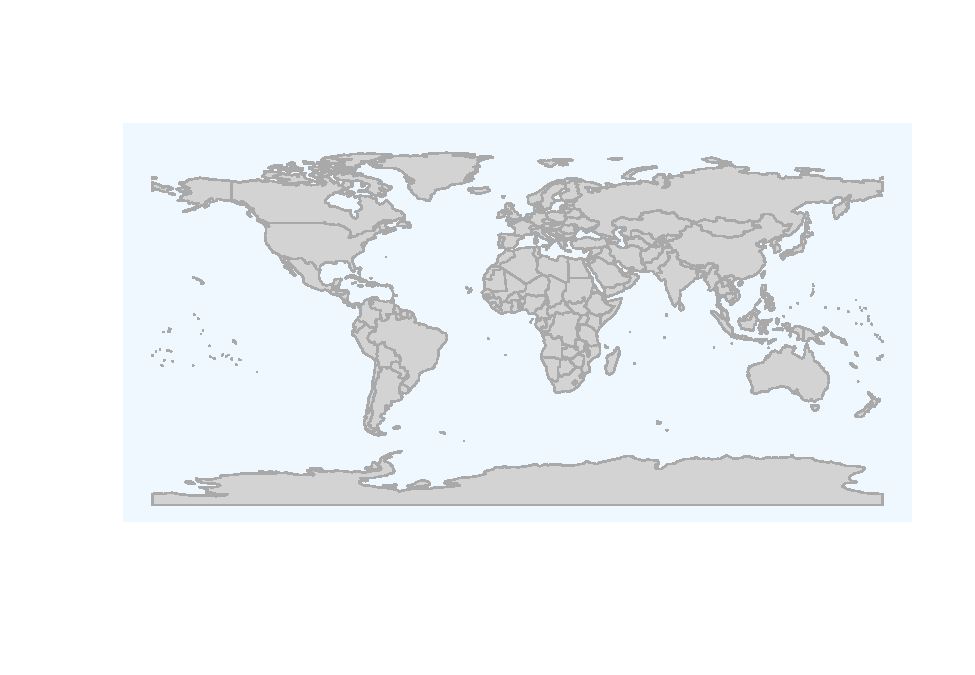
\includegraphics{EE_R-R_files/figure-pdf/unnamed-chunk-2-1.pdf}

}

\end{figure}

\begin{Shaded}
\begin{Highlighting}[]
\FunctionTok{library}\NormalTok{(countrycode)}
\FunctionTok{load}\NormalTok{(}\StringTok{"dat\_anal.RData"}\NormalTok{)}

\NormalTok{ClimatePolicy\_anal }\SpecialCharTok{\%\textgreater{}\%} 
  \FunctionTok{distinct}\NormalTok{(iso2c,}\AttributeTok{.keep\_all =}\NormalTok{ T) }\SpecialCharTok{\%\textgreater{}\%}
\NormalTok{  dplyr}\SpecialCharTok{::}\FunctionTok{select}\NormalTok{(iso2c,TargetSet) }\SpecialCharTok{\%\textgreater{}\%}
  \FunctionTok{mutate}\NormalTok{(}\AttributeTok{Type=}\FunctionTok{if\_else}\NormalTok{(TargetSet}\SpecialCharTok{==}\DecValTok{1}\NormalTok{,}\StringTok{"Target setting country"}\NormalTok{,}\StringTok{"Non{-}target setting country"}\NormalTok{))}\OtherTok{{-}\textgreater{}}\NormalTok{ countries}
\CommentTok{\# countries \%\textgreater{}\%}
\CommentTok{\#   as.data.frame() \%\textgreater{}\%}
\CommentTok{\#   head(15) \%\textgreater{}\%}
\CommentTok{\#   flextable() \%\textgreater{}\%}
\CommentTok{\#   flextable::set\_table\_properties(width = .5, layout = "autofit") \%\textgreater{}\%}
\CommentTok{\#   flextable::theme\_zebra() \%\textgreater{}\%}
\CommentTok{\#   flextable::fontsize(size = 12) \%\textgreater{}\%}
\CommentTok{\#   flextable::fontsize(size = 12, part = "header") \%\textgreater{}\%}
\CommentTok{\#   flextable::align\_text\_col(align = "center") \%\textgreater{}\%}
\CommentTok{\#   flextable::set\_caption(caption = "First 15 rows of the country codes.")  \%\textgreater{}\%}
\CommentTok{\#   flextable::border\_outer()}
\end{Highlighting}
\end{Shaded}

\begin{Shaded}
\begin{Highlighting}[]
\CommentTok{\# combine data frame with map}
\NormalTok{visitedMap }\OtherTok{\textless{}{-}} \FunctionTok{joinCountryData2Map}\NormalTok{(countries, }
                                  \AttributeTok{joinCode =} \StringTok{"ISO2"}\NormalTok{,}
                                  \AttributeTok{nameJoinColumn =} \StringTok{"iso2c"}\NormalTok{)}
\end{Highlighting}
\end{Shaded}

\begin{verbatim}
105 codes from your data successfully matched countries in the map
0 codes from your data failed to match with a country code in the map
137 codes from the map weren't represented in your data
\end{verbatim}

\begin{Shaded}
\begin{Highlighting}[]
\CommentTok{\# def. map parameters, e.g. def. colors}
\NormalTok{mapParams }\OtherTok{\textless{}{-}} \FunctionTok{mapCountryData}\NormalTok{(visitedMap, }
                            \AttributeTok{nameColumnToPlot=}\StringTok{"Type"}\NormalTok{,}
                            \AttributeTok{oceanCol =} \StringTok{"azure2"}\NormalTok{,}
                            \AttributeTok{catMethod =} \StringTok{"categorical"}\NormalTok{,}
                            \AttributeTok{missingCountryCol =} \FunctionTok{gray}\NormalTok{(.}\DecValTok{8}\NormalTok{),}
                            \AttributeTok{colourPalette =} \FunctionTok{c}\NormalTok{(}\StringTok{"coral"}\NormalTok{),}
                            \AttributeTok{addLegend =}\NormalTok{ F,}
                            \AttributeTok{mapTitle =} \StringTok{""}\NormalTok{,}
                            \AttributeTok{border =} \ConstantTok{NA}\NormalTok{)}
\end{Highlighting}
\end{Shaded}

\begin{verbatim}
Warning in rwmGetColours(colourPalette, numColours): colourPalette should be set to either a vector of colours or one of :white2Black black2White palette heat topo terrain rainbow negpos8 negpos9 
setting to heat colours as default
\end{verbatim}

\begin{Shaded}
\begin{Highlighting}[]
\CommentTok{\# add legend and display map}
\FunctionTok{do.call}\NormalTok{(addMapLegendBoxes, }\FunctionTok{c}\NormalTok{(mapParams,}
                             \AttributeTok{x =} \StringTok{\textquotesingle{}bottom\textquotesingle{}}\NormalTok{,}
                             \AttributeTok{title =} \StringTok{""}\NormalTok{,}
                             \AttributeTok{horiz =} \ConstantTok{TRUE}\NormalTok{,}
                             \AttributeTok{bg =} \StringTok{"transparent"}\NormalTok{,}
                             \AttributeTok{bty =} \StringTok{"n"}\NormalTok{))}
\end{Highlighting}
\end{Shaded}

\begin{figure}[H]

{\centering 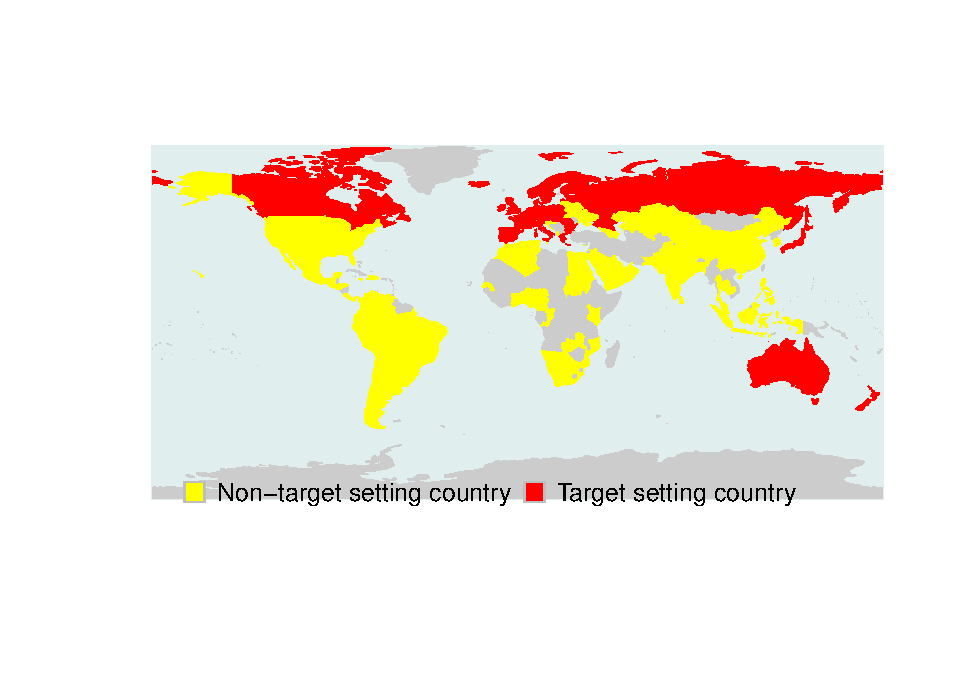
\includegraphics{EE_R-R_files/figure-pdf/fig-map-1.pdf}

}

\caption{\label{fig-map}Map of target setting countries}

\end{figure}

Table (\textbf{tab-1?}) shows the summary statistics of the variables
entering the model. These statistics reveal that significant variation
in outputs and inputs highlights considerable cross-sectional
heterogeneity. The variation is not surprising given the mix of
countries outlined Figure~\ref{fig-map}{[}\^{}12{]}.

{[}\^{}12{]}: Notice that some countries have a trade which exceeds GDP
(more than 100\%). This excess is usually a feature of small countries
with high productivity. Due to their small size, instead of being
self-sufficient and producing all the products their population needs,
they specialize in a few highly profitable industries. These industries
may produce more money from exports than the entire domestic economy,
which allows them to purchase imports far above what their domestic
economy could otherwise support. For example, in the sample, three
countries have a Trade to GDP ratio of over 200\%; Luxembourg, Malta and
Singapore.

\begin{Shaded}
\begin{Highlighting}[]
\NormalTok{sumThatFinal}\OtherTok{\textless{}{-}}\ControlFlowTok{function}\NormalTok{(x)\{}
\NormalTok{  p5}\OtherTok{=}\FunctionTok{quantile}\NormalTok{(x,}\AttributeTok{na.rm =}\NormalTok{ T,}\FloatTok{0.05}\NormalTok{)}
\NormalTok{  Median}\OtherTok{=}\FunctionTok{median}\NormalTok{(x,}\AttributeTok{na.rm =}\NormalTok{ T)}
\NormalTok{  Mean}\OtherTok{=}\FunctionTok{mean}\NormalTok{(x,}\AttributeTok{na.rm =}\NormalTok{ T)}
\NormalTok{  SD}\OtherTok{=}\FunctionTok{sd}\NormalTok{(x,}\AttributeTok{na.rm =}\NormalTok{ T)}
\NormalTok{  p95}\OtherTok{=}\FunctionTok{quantile}\NormalTok{(x,}\AttributeTok{na.rm =}\NormalTok{ T,}\FloatTok{0.95}\NormalTok{)}
  \FunctionTok{round}\NormalTok{(}\FunctionTok{c}\NormalTok{(Mean,SD,p5,Median,p95),}\DecValTok{2}\NormalTok{)}
\NormalTok{\}}

\NormalTok{sumStats}\OtherTok{\textless{}{-}}\NormalTok{ClimatePolicy\_anal }\SpecialCharTok{\%\textgreater{}\%} 
  \FunctionTok{as\_tibble}\NormalTok{() }\SpecialCharTok{\%\textgreater{}\%}
\NormalTok{  dplyr}\SpecialCharTok{::}\FunctionTok{select}\NormalTok{(CO2,y1,x2,x1,z1,z2,z3) }\SpecialCharTok{\%\textgreater{}\%} 
  \FunctionTok{group\_by}\NormalTok{(z3) }\SpecialCharTok{\%\textgreater{}\%} 
  \FunctionTok{summarise}\NormalTok{(}\FunctionTok{across}\NormalTok{(}\AttributeTok{.fns =}\NormalTok{ sumThatFinal)) }\SpecialCharTok{\%\textgreater{}\%}\NormalTok{ t}
\end{Highlighting}
\end{Shaded}

\begin{verbatim}
`summarise()` has grouped output by 'z3'. You can override using the `.groups`
argument.
\end{verbatim}

\begin{Shaded}
\begin{Highlighting}[]
\NormalTok{sumStats}\OtherTok{\textless{}{-}}\NormalTok{sumStats[}\SpecialCharTok{{-}}\DecValTok{1}\NormalTok{,}\FunctionTok{c}\NormalTok{(}\DecValTok{1}\NormalTok{,}\DecValTok{6}\NormalTok{,}\DecValTok{2}\NormalTok{,}\DecValTok{7}\NormalTok{,}\DecValTok{3}\NormalTok{,}\DecValTok{8}\NormalTok{,}\DecValTok{4}\NormalTok{,}\DecValTok{9}\NormalTok{,}\DecValTok{5}\NormalTok{,}\DecValTok{10}\NormalTok{)]}
\FunctionTok{rownames}\NormalTok{(sumStats)}\OtherTok{\textless{}{-}}\FunctionTok{c}\NormalTok{(}\StringTok{"C02 emissions (Million Metric Tons)"}\NormalTok{,}\StringTok{"GDP (Billion PPP $USD)"}\NormalTok{,}\StringTok{"Labour Force (Millions)"}\NormalTok{,}\StringTok{"Capital Stock (Billions PPP $USD)"}\NormalTok{,}\StringTok{"Urban to Total Population (\%)"}\NormalTok{,}\StringTok{"Trade to GDP (\%)"}\NormalTok{)}

\NormalTok{sumStats }\SpecialCharTok{\%\textgreater{}\%} 
  \FunctionTok{kable}\NormalTok{(}\StringTok{"latex"}\NormalTok{,}\AttributeTok{booktabs=}\NormalTok{T, }\AttributeTok{longtable=}\NormalTok{T,}\AttributeTok{caption =} \StringTok{"Summary statistics of inputs, outputs and z variables"}\NormalTok{,}\AttributeTok{align =} \StringTok{"c"}\NormalTok{,}\AttributeTok{row.names =}\NormalTok{T,}\AttributeTok{col.names =}\FunctionTok{rep}\NormalTok{(}\FunctionTok{c}\NormalTok{(}\StringTok{"Non Target"}\NormalTok{,}\StringTok{"Target"}\NormalTok{),}\DecValTok{5}\NormalTok{))  }\SpecialCharTok{\%\textgreater{}\%} 
  \FunctionTok{kable\_styling}\NormalTok{(}\AttributeTok{latex\_options =}\FunctionTok{c}\NormalTok{(}\StringTok{"HOLD\_position"}\NormalTok{), }\AttributeTok{font\_size =} \DecValTok{8}\NormalTok{, }\AttributeTok{full\_width=}\NormalTok{T) }\SpecialCharTok{\%\textgreater{}\%} 
  \FunctionTok{add\_header\_above}\NormalTok{(}\AttributeTok{header =}\FunctionTok{c}\NormalTok{(}\StringTok{" "}\OtherTok{=}\DecValTok{1}\NormalTok{,}\StringTok{"Mean"}\OtherTok{=}\DecValTok{2}\NormalTok{,}\StringTok{"StdDev"}\OtherTok{=}\DecValTok{2}\NormalTok{,}\StringTok{"5th\%ile"}\OtherTok{=}\DecValTok{2}\NormalTok{,}\StringTok{"Median"}\OtherTok{=}\DecValTok{2}\NormalTok{,}\StringTok{"95th\%ile"}\OtherTok{=}\DecValTok{2}\NormalTok{)) }\SpecialCharTok{\%\textgreater{}\%}
  \FunctionTok{column\_spec}\NormalTok{(}\DecValTok{1}\NormalTok{,}\AttributeTok{width=}\StringTok{"10em"}\NormalTok{) }\SpecialCharTok{\%\textgreater{}\%}
\NormalTok{ kableExtra}\SpecialCharTok{::}\FunctionTok{add\_footnote}\NormalTok{(}\AttributeTok{label=}\StringTok{"This table provides central tendency and spread statistics for the model variables for the sample period by target setting groups. Variables are presented on the measurement basis with which they enter the model, for example Capital stock enters the model in constant $Billions."}\NormalTok{,}\AttributeTok{threeparttable=}\NormalTok{T)}
\end{Highlighting}
\end{Shaded}

\begingroup\fontsize{8}{10}\selectfont

\begin{longtabu} to \linewidth {>{\raggedright\arraybackslash}p{10em}>{\centering}X>{\centering}X>{\centering}X>{\centering}X>{\centering}X>{\centering}X>{\centering}X>{\centering}X>{\centering}X>{\centering}X}
\begin{threeparttable}
\caption{Summary statistics of inputs, outputs and z variables}\\
\toprule
\multicolumn{1}{c}{ } & \multicolumn{2}{c}{Mean} & \multicolumn{2}{c}{StdDev} & \multicolumn{2}{c}{5th\%ile} & \multicolumn{2}{c}{Median} & \multicolumn{2}{c}{95th\%ile} \\
\cmidrule(l{3pt}r{3pt}){2-3} \cmidrule(l{3pt}r{3pt}){4-5} \cmidrule(l{3pt}r{3pt}){6-7} \cmidrule(l{3pt}r{3pt}){8-9} \cmidrule(l{3pt}r{3pt}){10-11}
  & Non Target & Target & Non Target & Target & Non Target & Target & Non Target & Target & Non Target & Target\\
\midrule
C02 emissions (Million Metric Tons) & 272.68 & 232.27 & 1086.07 & 346.03 & 2.24 & 7.72 & 22.30 & 66.70 & 496.12 & 1105.97\\
GDP (Billion PPP \$USD) & 764.05 & 910.94 & 2368.19 & 1159.91 & 16.10 & 33.56 & 113.62 & 362.44 & 2662.15 & 3432.20\\
Labour Force (Millions) & 31.82 & 13.60 & 105.78 & 18.58 & 0.81 & 0.24 & 5.53 & 4.94 & 113.96 & 66.18\\
Capital Stock (Billions PPP \$USD) & 1552.25 & 2133.53 & 5168.49 & 2937.17 & 20.80 & 69.57 & 170.11 & 919.89 & 5832.42 & 7321.33\\
Urban to Total Population (\%) & 60.32 & 75.83 & 21.00 & 11.44 & 24.15 & 54.88 & 59.75 & 77.00 & 94.21 & 93.53\\
\addlinespace
Trade to GDP (\%) & 88.35 & 99.64 & 55.18 & 57.63 & 34.16 & 43.18 & 75.73 & 84.75 & 158.02 & 181.70\\
\bottomrule
\end{longtabu}
\endgroup{}

\hypertarget{results-and-discussion}{%
\section{Results and Discussion}\label{results-and-discussion}}

We estimate a step-wise yield curve of probabilistic benchmark
technologies. These technologies extract, at the observed performance
level, country-year marginal abatement costs of CO\textsubscript{2}
emissions. We use the direction vector to estimate the directional
distance function model for 10 quantiles, which should be sufficient
granularity for a sample size of 525. Finally, we include a noise term
that captures measurement errors in the data.

\begin{Shaded}
\begin{Highlighting}[]
\NormalTok{ClimatePolicy\_anal }\SpecialCharTok{\%\textgreater{}\%} 
  \FunctionTok{group\_by}\NormalTok{(year) }\SpecialCharTok{\%\textgreater{}\%}
  \FunctionTok{summarise}\NormalTok{(}\StringTok{"MAC Overall"}\OtherTok{=}\FunctionTok{mean}\NormalTok{(MAC,}\AttributeTok{na.rm =}\NormalTok{ T),}
            \StringTok{"IQR"}\OtherTok{=}\FunctionTok{IQR}\NormalTok{(MAC,}\AttributeTok{na.rm =}\NormalTok{ T),}
            \StringTok{"MAC Target Setters"}\OtherTok{=}\FunctionTok{mean}\NormalTok{(MAC\_T,}\AttributeTok{na.rm =}\NormalTok{ T),}
            \StringTok{"IQR1"}\OtherTok{=}\FunctionTok{IQR}\NormalTok{(MAC\_T,}\AttributeTok{na.rm =}\NormalTok{ T),}
            \StringTok{"MAC Non Target Setters"}\OtherTok{=}\FunctionTok{mean}\NormalTok{(MAC\_No\_T,}\AttributeTok{na.rm =}\NormalTok{ T),}
            \StringTok{"IQR2"}\OtherTok{=}\FunctionTok{IQR}\NormalTok{(MAC\_No\_T,}\AttributeTok{na.rm =}\NormalTok{ T)) }\SpecialCharTok{\%\textgreater{}\%}
  \FunctionTok{kable}\NormalTok{(}\StringTok{"latex"}\NormalTok{,}\AttributeTok{digits =} \DecValTok{2}\NormalTok{,}\AttributeTok{caption =} \StringTok{"Marginal abatement costs in 2011 dollars per CO2 tonne"}\NormalTok{,}\AttributeTok{align =} \StringTok{"c"}\NormalTok{,}\AttributeTok{booktabs=}\NormalTok{T,}\AttributeTok{col.names =} \FunctionTok{c}\NormalTok{(}\StringTok{""}\NormalTok{,}\FunctionTok{rep}\NormalTok{(}\FunctionTok{c}\NormalTok{(}\StringTok{"Mean"}\NormalTok{,}\StringTok{"Interquartile Range"}\NormalTok{),}\DecValTok{3}\NormalTok{)),}\AttributeTok{longtable=}\NormalTok{T) }\SpecialCharTok{\%\textgreater{}\%}
  \FunctionTok{kable\_styling}\NormalTok{(}\AttributeTok{font\_size=}\DecValTok{8}\NormalTok{,}\AttributeTok{latex\_options =}\FunctionTok{c}\NormalTok{(}\StringTok{"hold\_position"}\NormalTok{), }\AttributeTok{full\_width=}\NormalTok{T) }\SpecialCharTok{\%\textgreater{}\%}
  \FunctionTok{add\_header\_above}\NormalTok{(}\FunctionTok{c}\NormalTok{(}\StringTok{""}\NormalTok{,}\StringTok{"Full Sample"}\OtherTok{=}\DecValTok{2}\NormalTok{,}\StringTok{"Target Setting Countries"}\OtherTok{=}\DecValTok{2}\NormalTok{,}\StringTok{"Non Target Setting Countries"}\OtherTok{=}\DecValTok{2}\NormalTok{),}\AttributeTok{bold =}\NormalTok{ T,}\AttributeTok{italic =}\NormalTok{ T) }\SpecialCharTok{\%\textgreater{}\%}
  \FunctionTok{row\_spec}\NormalTok{(}\DecValTok{0}\NormalTok{,}\AttributeTok{bold =}\NormalTok{ T,}\AttributeTok{italic =}\NormalTok{ T)  }\SpecialCharTok{\%\textgreater{}\%}
  \FunctionTok{add\_footnote}\NormalTok{(}\AttributeTok{label=}\StringTok{"This table presents yearly mean and interquartile estimates of the marginal abatement costs calculated for the full sample and for each group of countries.  The last four columns disaggregates the mean analysis to compare countries which set emission reduction targets against countries which did not.  GDP(y) and capital stock (x1) are deflated to 2011 international dollars, and are considered to have a unit price.  An alternative interpretation is that the the price multipliers (p,w)=1 in the calculations of the marginal rate of transformation of GDP and the marginal product of the capital stock as they represent both quantity and price. The marginal abatement cost is thus calculated as the minimum of the marginal rate of transformation of GDP and the marginal product of capital stock on C0\textasciitilde{}2\textasciitilde{} emissions.  The MAC is measured in USD per metric ton of CO\textasciitilde{}2\textasciitilde{} emission. Labour (x2) is the total labour force in each country (in millions).  The marginal product of labour is the dual without a price multiplier and is measured in millions of labour force per ton of CO2 emission."}\NormalTok{,}\AttributeTok{threeparttable=}\NormalTok{T)}
\end{Highlighting}
\end{Shaded}

\begingroup\fontsize{8}{10}\selectfont

\begin{longtabu} to \linewidth {>{\centering}X>{\centering}X>{\centering}X>{\centering}X>{\centering}X>{\centering}X>{\centering}X}
\begin{threeparttable}
\caption{Marginal abatement costs in 2011 dollars per CO2 tonne}\\
\toprule
\multicolumn{1}{c}{\em{\textbf{}}} & \multicolumn{2}{c}{\em{\textbf{Full Sample}}} & \multicolumn{2}{c}{\em{\textbf{Target Setting Countries}}} & \multicolumn{2}{c}{\em{\textbf{Non Target Setting Countries}}} \\
\cmidrule(l{3pt}r{3pt}){2-3} \cmidrule(l{3pt}r{3pt}){4-5} \cmidrule(l{3pt}r{3pt}){6-7}
\em{\textbf{}} & \em{\textbf{Mean}} & \em{\textbf{Interquartile Range}} & \em{\textbf{Mean}} & \em{\textbf{Interquartile Range}} & \em{\textbf{Mean}} & \em{\textbf{Interquartile Range}}\\
\midrule
2008 & 71.91 & 53.59 & 64.45 & 46.22 & 74.95 & 55.35\\
2009 & 81.18 & 63.47 & 90.09 & 40.74 & 77.64 & 63.37\\
2010 & 87.89 & 72.61 & 95.93 & 53.77 & 84.19 & 75.52\\
2011 & 86.73 & 60.64 & 89.64 & 51.83 & 85.46 & 84.99\\
2012 & 103.31 & 67.47 & 111.07 & 75.47 & 100.23 & 58.25\\
\bottomrule
\end{longtabu}
\endgroup{}

Table (\textbf{tab-macdiff?}) summarises the marginal abatement cost
estimates for each year in our sample period. This table presents the
mean and interquartile range for the entire sample, targeting setting
countries and their non-target setting counterparts. Marginal abatement
costs illustrate the carbon intensity, where countries with larger
manufacturing sectors will have relatively higher MAC estimates. The MAC
estimates are similar to those reported in the literature (Lee, Oh, and
Lee 2014; Böhringer and Vogt 2003; Viguier, Babiker, and Reilly 2003) ,
and comparatively similar to the cost of C0\textsubscript{2} capture and
storage of coal plants estimated by Rubin, Davison, and Herzog (2015) ,
who estimates a mitigation cost (constant 2013 dollar per metric tonne
of CO2) for the capture of 46-99 US dollars and storage of 53-137 US
dollars.

\hypertarget{carbon-emissions-pricing-comparison}{%
\subsection{Carbon emissions pricing
comparison}\label{carbon-emissions-pricing-comparison}}

There is a common theoretical starting point for carbon emissions
pricing and carbon shadow pricing, a sufficiently high emissions price
for imposing zero emissions that cause global warming. An appropriate
carbon pricing regime should treat these two options as mutually
reinforcing. Carbon emission pricing being where policymakers add a
carbon component to the current market price of pollutants. Shadow
pricing being where policymakers ascertains a future price of the actual
economic cost of a climate-relevant project. Both have a real-world
impact in that they drive markets towards factoring in long-term
impacts. In practice, the pricing schemes diverge due to political
inconvenience and inadequate multilateral commitments (Hans-Jochen,
Sabine, and Hans 2020)

Since the introduction of the KP, emission pricing schemes are political
motivators to state actors, where it is politically inconvenient to
increase such tax in line with climate impacts. While efforts such as
the EU emission trading scheme, introduced in 2008 for major industrial
facilities, have been shown to only cover about 40\% of the European
greenhouse-gas emissions . In contrast, shadow pricing essentially
bypasses national governments, as it is commonly used by multilateral
development banks. At present, only projects in emerging and developing
countries routinely apply shadow pricing(Hans-Jochen, Sabine, and Hans
2020). The approach essentially adopted here is a social value of carbon
(SVC). The Stiglitz et al. (2017) report on carbon prices established an
SVC shadow price range necessary to achieve the Paris temperature target
as \$40-80/tCO2 by 2020, and \$50-100/tCO2 by 2030.

\begin{Shaded}
\begin{Highlighting}[]
\FunctionTok{library}\NormalTok{(readxl)}
\FunctionTok{library}\NormalTok{(dplyr)}
\FunctionTok{read\_excel}\NormalTok{(}\StringTok{"CPI\_Data\_DashboardExtract.xlsx"}\NormalTok{,}
           \AttributeTok{sheet =} \StringTok{"Data\_Price"}\NormalTok{,}
           \AttributeTok{skip =} \DecValTok{2}\NormalTok{,}\AttributeTok{na=}\StringTok{"N/A"}\NormalTok{) }\OtherTok{{-}\textgreater{}}\NormalTok{df}
\NormalTok{df }\OtherTok{\textless{}{-}}\NormalTok{ df[,}\FunctionTok{colSums}\NormalTok{(}\FunctionTok{is.na}\NormalTok{(df))}\SpecialCharTok{\textless{}}\FunctionTok{nrow}\NormalTok{(df)]}
\NormalTok{df }\SpecialCharTok{\%\textgreater{}\%} \FunctionTok{filter}\NormalTok{(}\StringTok{\textasciigrave{}}\AttributeTok{Name of the initiative}\StringTok{\textasciigrave{}}\SpecialCharTok{==}\StringTok{"EU ETS"}\NormalTok{)}\OtherTok{{-}\textgreater{}}\NormalTok{df}
\NormalTok{df }\SpecialCharTok{\%\textgreater{}\%} 
\NormalTok{  dplyr}\SpecialCharTok{::}\FunctionTok{select}\NormalTok{(}\SpecialCharTok{{-}}\StringTok{\textasciigrave{}}\AttributeTok{Jurisdiction Covered}\StringTok{\textasciigrave{}}\NormalTok{,}\SpecialCharTok{{-}}\StringTok{\textasciigrave{}}\AttributeTok{Instrument Type}\StringTok{\textasciigrave{}}\NormalTok{) }\SpecialCharTok{\%\textgreater{}\%}
  \FunctionTok{gather}\NormalTok{(Year,Price\_USD\_2011,}\SpecialCharTok{{-}}\StringTok{\textasciigrave{}}\AttributeTok{Name of the initiative}\StringTok{\textasciigrave{}}\NormalTok{) }\SpecialCharTok{\%\textgreater{}\%}
  \FunctionTok{mutate}\NormalTok{(}\AttributeTok{Year=}\FunctionTok{as.numeric}\NormalTok{(}\FunctionTok{str\_replace}\NormalTok{(Year,}\StringTok{"Price\_rate\_1\_"}\NormalTok{,}\StringTok{""}\NormalTok{)),}
         \AttributeTok{Price\_USD\_2011=}\FunctionTok{as.numeric}\NormalTok{(Price\_USD\_2011)) }\SpecialCharTok{\%\textgreater{}\%}
  \FunctionTok{rename}\NormalTok{(}\AttributeTok{Initiative=}\StringTok{"Name of the initiative"}\NormalTok{) }\SpecialCharTok{\%\textgreater{}\%}
  \FunctionTok{filter}\NormalTok{(Year}\SpecialCharTok{\textgreater{}=}\DecValTok{2008}\NormalTok{) }\SpecialCharTok{\%\textgreater{}\%}
  \FunctionTok{rbind}\NormalTok{(}
\NormalTok{  ClimatePolicy\_anal }\SpecialCharTok{\%\textgreater{}\%} 
  \FunctionTok{group\_by}\NormalTok{(year) }\SpecialCharTok{\%\textgreater{}\%}
  \FunctionTok{summarise}\NormalTok{(}\StringTok{"Shadow Price KP target{-}setters"}\OtherTok{=}\FunctionTok{mean}\NormalTok{(MAC\_T,}\AttributeTok{na.rm =}\NormalTok{ T),          }
            \StringTok{"Shadow Price KP non{-} target setters"}\OtherTok{=}\FunctionTok{mean}\NormalTok{(MAC\_No\_T,}\AttributeTok{na.rm =}\NormalTok{ T)) }\SpecialCharTok{\%\textgreater{}\%} \FunctionTok{rename}\NormalTok{(}\AttributeTok{Year=}\NormalTok{year) }\SpecialCharTok{\%\textgreater{}\%}
    \FunctionTok{gather}\NormalTok{(Initiative,Price\_USD\_2011,}\SpecialCharTok{{-}}\NormalTok{Year)) }\SpecialCharTok{\%\textgreater{}\%}
  \FunctionTok{ggplot}\NormalTok{(}\FunctionTok{aes}\NormalTok{(}\AttributeTok{x=}\FunctionTok{as.character}\NormalTok{(Year),}\AttributeTok{y=}\NormalTok{Price\_USD\_2011,}\AttributeTok{group=}\NormalTok{Initiative)) }\SpecialCharTok{+}
  \FunctionTok{geom\_point}\NormalTok{(}\FunctionTok{aes}\NormalTok{(}\AttributeTok{shape=}\NormalTok{Initiative,}\AttributeTok{colour=}\NormalTok{Initiative)) }\SpecialCharTok{+}
  \FunctionTok{geom\_line}\NormalTok{(}\FunctionTok{aes}\NormalTok{(}\AttributeTok{colour=}\NormalTok{Initiative),}\AttributeTok{linetype=}\StringTok{"dotdash"}\NormalTok{) }\SpecialCharTok{+}
  \FunctionTok{labs}\NormalTok{(}\AttributeTok{x=}\StringTok{""}\NormalTok{, }\AttributeTok{y=}\StringTok{"US$/tCO2e"}\NormalTok{,}\AttributeTok{caption =} \StringTok{"Source: World Bank Carbon Pricing Dashboard"}\NormalTok{) }\SpecialCharTok{+}
  \CommentTok{\# coord\_flip() +}
  \FunctionTok{theme}\NormalTok{(}
    \AttributeTok{text =} \FunctionTok{element\_text}\NormalTok{(}\AttributeTok{size=}\DecValTok{20}\NormalTok{),}
        \AttributeTok{legend.position =} \StringTok{"top"}
\NormalTok{       ,}\AttributeTok{legend.text =} \FunctionTok{element\_text}\NormalTok{(}\AttributeTok{size=}\DecValTok{15}\NormalTok{)}
\NormalTok{        ) }\SpecialCharTok{+}
  \FunctionTok{scale\_fill\_brewer}\NormalTok{(}\AttributeTok{type =} \StringTok{"qual"}\NormalTok{)}
\end{Highlighting}
\end{Shaded}

\begin{figure}[H]

{\centering 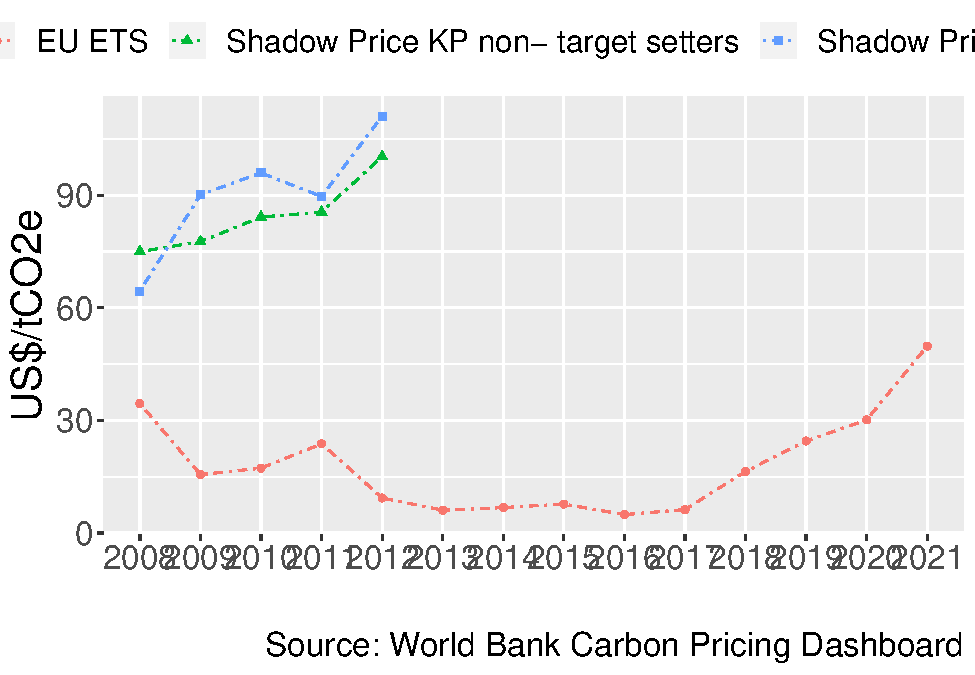
\includegraphics{EE_R-R_files/figure-pdf/fig-ets-1.pdf}

}

\caption{\label{fig-ets}\textbf{?(caption)}}

\end{figure}

Figure Figure~\ref{fig-ets} compares the 2011 nominal Carbon Prices from
the EU emission trading schemes (ETS) to our shadow price mean
estimates. Over the four years of the KP, the shadow price for both
groups (target setting and non-target setting) is a multiple of the
prices from the ETS. While our estimates trend up over the period the
ETS prices actually fall. In keeping with Hans-Jochen, Sabine, and Hans
(2020) forward looking definition of shadow prices, in the last year the
EU-ETS price has increased dramatically and is beginning to approach our
shadow price estimates.

For an emissions trading scheme to work efficiently, allocation of
abatement across countries would require that the marginal abatement
cost is the same in all countries and over time. The results from table
(\textbf{tab-2?}) suggest this is not the case. The mean MAC is trending
up in both groupings and is typically most significant for target
setting countries. Furthermore, the EU-ETS market, which allows firms
from different countries to buy and sell CO\textsubscript{2} emission
allowances to achieve an efficient allocation of abatement, is not
working to lower the marginal abatement costs of the period. This visual
argument suggests a consistent sub-optimal allocation of
CO\textsubscript{2} abatement across countries and significant frictions
in ETS market price discovery.

\hypertarget{marginal-effect-of-the-environmental-variable}{%
\subsection{Marginal effect of the environmental
variable}\label{marginal-effect-of-the-environmental-variable}}

Following Gallagher and Quinn (2019), we investigate the marginal effect
of the environmental variables in equation \textbf{?@eq-1} to understand
how they impact inefficiency. Specifically, we consider how inefficiency
is affected by the proportion of trade to GDP, the percentage of the
urban living in a country's population, and whether the country
explicitly sets CO\textsubscript{2} emission targets in the analysis
period.

\begin{Shaded}
\begin{Highlighting}[]
\NormalTok{ClimatePolicy\_anal }\SpecialCharTok{\%\textgreater{}\%} \FunctionTok{mutate}\NormalTok{(}\AttributeTok{logGDP=}\FunctionTok{log}\NormalTok{(GDP),}
                   \AttributeTok{logx=}\FunctionTok{log}\NormalTok{((Capital}\SpecialCharTok{+}\NormalTok{LABOUR}\SpecialCharTok{+}\NormalTok{CO2)}\SpecialCharTok{/}\DecValTok{3}\SpecialCharTok{+}\DecValTok{1}\NormalTok{),}
                   \AttributeTok{regY=}\NormalTok{logGDP}\SpecialCharTok{{-}}\NormalTok{logx,}
                   \AttributeTok{Yr=}\FunctionTok{as.factor}\NormalTok{(year),}
                   \AttributeTok{Setter=}\FunctionTok{as.factor}\NormalTok{(TargetSet)) }\SpecialCharTok{\%\textgreater{}\%}
\NormalTok{  dplyr}\SpecialCharTok{::}\FunctionTok{select}\NormalTok{(regY,TRADEtoGDP,URBAN,Setter,Yr,country) }\OtherTok{{-}\textgreater{}}\NormalTok{df\_anal}

\FunctionTok{lm}\NormalTok{(regY}\SpecialCharTok{\textasciitilde{}}\NormalTok{TRADEtoGDP}\SpecialCharTok{+}\NormalTok{URBAN}\SpecialCharTok{+}\NormalTok{Setter}\SpecialCharTok{+}\NormalTok{Yr,}\AttributeTok{data=}\NormalTok{df\_anal) }\SpecialCharTok{\%\textgreater{}\%}
  \FunctionTok{tidy}\NormalTok{() }\SpecialCharTok{\%\textgreater{}\%}
  \CommentTok{\# mutate(estimate=exp(estimate))}
  \FunctionTok{slice}\NormalTok{(}\SpecialCharTok{{-}}\DecValTok{1}\NormalTok{) }\SpecialCharTok{\%\textgreater{}\%}
  \FunctionTok{kable}\NormalTok{(}\StringTok{"latex"}\NormalTok{,}\AttributeTok{digits =} \DecValTok{3}\NormalTok{,}\AttributeTok{caption =} \StringTok{"Marginal effect of enviromental variables"}\NormalTok{,}\AttributeTok{align =} \StringTok{"c"}\NormalTok{,}\AttributeTok{booktabs=}\NormalTok{T,}\AttributeTok{longtable=}\NormalTok{T) }\SpecialCharTok{\%\textgreater{}\%}
  \FunctionTok{add\_footnote}\NormalTok{(}\AttributeTok{label=}\StringTok{"This table shows the marginal effects from the z coefficients in equation (1) by exploiting statistical procedure first outlined in Kuosmenan \& Johnson (2015)."}\NormalTok{,}\AttributeTok{threeparttable =}\NormalTok{ T) }\SpecialCharTok{\%\textgreater{}\%}
  \FunctionTok{kable\_styling}\NormalTok{(}\AttributeTok{full\_width =}\NormalTok{ T)}
\end{Highlighting}
\end{Shaded}

\begin{verbatim}
Warning in add_footnote(., label = "This table shows the marginal effects from
the z coefficients in equation (1) by exploiting statistical procedure first
outlined in Kuosmenan & Johnson (2015).", : Notation is set to 'number' and
other formats are not supported.
\end{verbatim}

\begin{verbatim}
Warning in add_footnote(., label = "This table shows the marginal effects from
the z coefficients in equation (1) by exploiting statistical procedure first
outlined in Kuosmenan & Johnson (2015).", : Threeparttable does not support
longtable.
\end{verbatim}

\begin{longtabu} to \linewidth {>{\centering}X>{\centering}X>{\centering}X>{\centering}X>{\centering}X}
\caption{Marginal effect of enviromental variables}\\
\toprule
term & estimate & std.error & statistic & p.value\\
\midrule
TRADEtoGDP & 0.002 & 0.000 & 4.567 & 0.000\\
URBAN & 0.031 & 0.001 & 23.856 & 0.000\\
Setter1 & 0.628 & 0.056 & 11.277 & 0.000\\
Yr2009 & -0.016 & 0.075 & -0.209 & 0.834\\
Yr2010 & -0.013 & 0.075 & -0.169 & 0.866\\
\addlinespace
Yr2011 & -0.014 & 0.075 & -0.191 & 0.849\\
Yr2012 & -0.016 & 0.075 & -0.216 & 0.829\\
\bottomrule
\end{longtabu}

The results from table (\textbf{tab-effects?}) reveal some interesting
features of the inefficient patterns at the country level. Typically,
those with higher trade to GDP ratios and higher urban populations tend
to be less efficient over the sample. Interestingly, those countries
which are setting targets tend to be more inefficient in the sample
period. Finally, there is an overall reduction in inefficiency over the
period indicated by the year dummies, although this relationship is not
significant in the data.

\hypertarget{shadow-price-differences}{%
\subsection{Shadow price differences}\label{shadow-price-differences}}

Our statistical shadow price difference test is based on the underlying
data for frontier efficiency. Specifically, it is the ratio of the
corresponding bad output to either good output or input that is
represented in a shadow price estimate. For example, the ratio of
CO\textsubscript{2} emissions to GDP could be used to test statistical
differences in the shadow price of the good output calculated as
\(MRT_{\tau}(y_{i},b_{j})=-\frac{\delta \vec{D}_{\tau}/\delta b_{j}}{\delta \vec{D}_{\tau}/\delta y_{i}}\).

\begin{Shaded}
\begin{Highlighting}[]
\FunctionTok{library}\NormalTok{(pander)}
\CommentTok{\# LeveneTest only works with factor variables in the formula}
\NormalTok{ClimatePolicy\_anal}\SpecialCharTok{$}\NormalTok{Target}\OtherTok{\textless{}{-}}\FunctionTok{as.factor}\NormalTok{(ClimatePolicy\_anal}\SpecialCharTok{$}\NormalTok{TargetSet)}
\NormalTok{ClimatePolicy\_anal }\OtherTok{\textless{}{-}}\NormalTok{ ClimatePolicy\_anal }\SpecialCharTok{\%\textgreater{}\%}\NormalTok{ as\_tibble}
\NormalTok{StatTest}\OtherTok{\textless{}{-}}\ControlFlowTok{function}\NormalTok{(df,x,netput,grp,start,end) \{}
\NormalTok{  p}\OtherTok{\textless{}{-}}\FunctionTok{c}\NormalTok{(start}\SpecialCharTok{:}\NormalTok{end)}
\NormalTok{  out}\OtherTok{\textless{}{-}}\FunctionTok{matrix}\NormalTok{(}\ConstantTok{NA}\NormalTok{,}\AttributeTok{nrow =}\FunctionTok{length}\NormalTok{(p),}\AttributeTok{ncol =}\DecValTok{8}\NormalTok{)}
  \ControlFlowTok{for}\NormalTok{ (i }\ControlFlowTok{in}\NormalTok{ p) \{}
\NormalTok{    dftest}\OtherTok{\textless{}{-}}\FunctionTok{subset}\NormalTok{(df,year}\SpecialCharTok{==}\NormalTok{i)}
\NormalTok{    j}\OtherTok{=}\NormalTok{i}\DecValTok{{-}2007}
    \CommentTok{\# Allows the function inputs to call the netput variable}
\NormalTok{    dftest}\SpecialCharTok{$}\NormalTok{ratio}\OtherTok{\textless{}{-}}\FunctionTok{eval}\NormalTok{(}\FunctionTok{substitute}\NormalTok{(x),dftest)}\SpecialCharTok{/}\FunctionTok{eval}\NormalTok{(}\FunctionTok{substitute}\NormalTok{(netput),dftest)}
\NormalTok{    TR}\OtherTok{\textless{}{-}}\NormalTok{dftest[}\FunctionTok{eval}\NormalTok{(}\FunctionTok{substitute}\NormalTok{(grp),dftest)}\SpecialCharTok{==}\DecValTok{1}\NormalTok{,]}\SpecialCharTok{$}\NormalTok{ratio}
\NormalTok{    CO}\OtherTok{\textless{}{-}}\NormalTok{dftest[}\FunctionTok{eval}\NormalTok{(}\FunctionTok{substitute}\NormalTok{(grp),dftest)}\SpecialCharTok{==}\DecValTok{0}\NormalTok{,]}\SpecialCharTok{$}\NormalTok{ratio}
    \CommentTok{\# Allows grp input to be called as a string}
\NormalTok{    f}\OtherTok{\textless{}{-}}\FunctionTok{as.formula}\NormalTok{(}\FunctionTok{paste0}\NormalTok{(}\StringTok{"ratio"}\NormalTok{,}\StringTok{"\textasciitilde{}"}\NormalTok{,}\FunctionTok{deparse}\NormalTok{(}\FunctionTok{substitute}\NormalTok{(grp))))}
    
\NormalTok{      out[j,}\DecValTok{1}\SpecialCharTok{:}\DecValTok{4}\NormalTok{]}\OtherTok{\textless{}{-}}\FunctionTok{c}\NormalTok{(}\FunctionTok{ad.test}\NormalTok{(dftest}\SpecialCharTok{$}\NormalTok{ratio)}\SpecialCharTok{$}\NormalTok{statistic,}
                    \FunctionTok{leveneTest}\NormalTok{(f,dftest,}\AttributeTok{center=}\NormalTok{mean)}\SpecialCharTok{$}\StringTok{\textasciigrave{}}\AttributeTok{F value}\StringTok{\textasciigrave{}}\NormalTok{[}\DecValTok{1}\NormalTok{],}
                    \FunctionTok{kruskal.test}\NormalTok{(f,dftest)}\SpecialCharTok{$}\NormalTok{statistic,}
                    \FunctionTok{ks.boot}\NormalTok{(TR,CO)}\SpecialCharTok{$}\NormalTok{ks}\SpecialCharTok{$}\NormalTok{statistic)}
      
\NormalTok{      out[j,}\DecValTok{5}\SpecialCharTok{:}\DecValTok{8}\NormalTok{]}\OtherTok{\textless{}{-}}\FunctionTok{c}\NormalTok{(}\FunctionTok{ad.test}\NormalTok{(dftest}\SpecialCharTok{$}\NormalTok{ratio)}\SpecialCharTok{$}\NormalTok{p.value,}
                    \FunctionTok{leveneTest}\NormalTok{(f,dftest,}\AttributeTok{center=}\NormalTok{mean)}\SpecialCharTok{$}\StringTok{\textasciigrave{}}\AttributeTok{Pr(\textgreater{}F)}\StringTok{\textasciigrave{}}\NormalTok{[}\DecValTok{1}\NormalTok{],}
                    \FunctionTok{kruskal.test}\NormalTok{(f,dftest)}\SpecialCharTok{$}\NormalTok{p.value,}
                    \FunctionTok{ks.boot}\NormalTok{(TR,CO)}\SpecialCharTok{$}\NormalTok{ks}\SpecialCharTok{$}\NormalTok{p.value)}
\NormalTok{  \}}
  \CommentTok{\# To produce a more statistical output required the additional of "stariness" to the out matrix using the pander function add.significance.stars}
\NormalTok{out}\OtherTok{\textless{}{-}}\FunctionTok{matrix}\NormalTok{(}\FunctionTok{paste0}\NormalTok{(}\FunctionTok{as.matrix}\NormalTok{(}\FunctionTok{round}\NormalTok{(out[,}\FunctionTok{c}\NormalTok{(}\DecValTok{1}\SpecialCharTok{:}\DecValTok{4}\NormalTok{)],}\DecValTok{2}\NormalTok{)),}\FunctionTok{as.matrix}\NormalTok{(}\FunctionTok{add.significance.stars}\NormalTok{(out[,}\FunctionTok{c}\NormalTok{(}\DecValTok{5}\SpecialCharTok{:}\DecValTok{8}\NormalTok{)]))),}\AttributeTok{nrow=}\FunctionTok{nrow}\NormalTok{(out))}
\FunctionTok{rownames}\NormalTok{(out)}\OtherTok{\textless{}{-}}\NormalTok{p}
\NormalTok{out}
\NormalTok{\}}

\FunctionTok{StatTest}\NormalTok{(ClimatePolicy\_anal,CO2,LABOUR,Target,}\DecValTok{2008}\NormalTok{,}\DecValTok{2012}\NormalTok{) }\SpecialCharTok{\%\textgreater{}\%}
  \FunctionTok{kable}\NormalTok{(}\AttributeTok{caption =} \StringTok{"Statistical Analysis of Marginal Abatement Cost Differences"}\NormalTok{,}\AttributeTok{align =} \StringTok{"c"}\NormalTok{, }\AttributeTok{col.names=}\FunctionTok{c}\NormalTok{(}\StringTok{"Normality Test"}\NormalTok{,}\StringTok{"Equality of Variance"}\NormalTok{,}\StringTok{"Rank sum z{-}test"}\NormalTok{,}\StringTok{"Equality of distribution D{-}test"}\NormalTok{)) }
\end{Highlighting}
\end{Shaded}

\begin{table}

\caption{Statistical Analysis of Marginal Abatement Cost Differences}
\centering
\begin{tabular}[t]{l|c|c|c|c}
\hline
  & Normality Test & Equality of Variance & Rank sum z-test & Equality of distribution D-test\\
\hline
2008 & 4.25 * * * & 2.83 & 25.8 * * * & 0.64 * * *\\
\hline
2009 & 4.3 * * * & 2.92 & 25.51 * * * & 0.62 * * *\\
\hline
2010 & 4.18 * * * & 2.29 & 25.58 * * * & 0.64 * * *\\
\hline
2011 & 4.2 * * * & 2.64 & 23.97 * * * & 0.62 * * *\\
\hline
2012 & 4.08 * * * & 2.95 & 23.09 * * * & 0.62 * * *\\
\hline
\end{tabular}
\end{table}

Table (\textbf{tab-stattest?}) shows the results of the testing approach
described in test steps applied each year to the ratio of the variables
represented by the MAC estimates. The first column presents the test
results of the empirical distribution of the ratio and shows that
normality is rejected for all years. This result implies that we should
use a nonparametric group difference test. Column 2 presents the
equality of variance test across the groups of interest, robust to
non-normal distribution. Equality of variance is not rejected for all
years. Columns 3 and 4 of table (\textbf{tab-stattest?}) provide a
statistical analysis of the observed mean differences in shadow prices
presented in table (\textbf{tab-macdiff?}) . In column 3, the Wilcoxon
Mann Whitney test provides robust inference when we cannot reject the
hypothesis of equality of variance in groups assessed in column 2. The
Kolmogorov Smirnov test provides robust inference if the equality of
variance hypothesis is rejected. Given the results of column 2, column 3
results suggest a statistically significant difference in the shadow
prices of the two cohorts. This finding provides some meaningful
evidence that target setting countries consistently experienced
increased abatement costs than non-target setting counties during the
Kyoto protocol period.

\hypertarget{concluding-remarks}{%
\section{Concluding remarks}\label{concluding-remarks}}

This study contributes to the ongoing debate on target setting
implications in climate policy. We use a frontier efficiency approach
which reveals unintended consequences of target setting in the first KP
commitment period (2008-2012). Target setters were less environmentally
efficient and had higher marginal abatement costs for CO 2 emissions. We
also note both international variation in marginal abatement costs as
well as variation between marginal abatement costs and market pricing of
carbon. Our findings have important implications for international
carbon regulation.

Firstly, in contrast to previous work, we show that the shadow price and
market price of CO\textsubscript{2} diverge in the KP period, suggestive
of a consistent misallocation of the traded allowances in the EU
emissions trading scheme (ETS).

Secondly, our results also show an imbalance in shadow pricing due to
target setting. For an emissions trading scheme to work efficiently,
marginal abatement costs across countries should be identical and equal
to the market clearing price of carbon. Recently, EU policymakers, to
control market instability, passed legislation that allows for a surplus
in carbon trading allowance due to the production shock of the COVID-19
pandemic. A structural consequence of our findings could also be a
surplus of allowances, exacerbating market instability, lowering the
carbon price, and weakening the incentives to reduce emissions. We argue
that market stability rules for surplus allowances must also consider
the heterogeneity in regional standards and targets for emission
abatement.

Encouragingly, although ignoring the trading period since the KP, in
recent years the emissions trading market price is beginning to approach
the lower end of our shadow price estimates which suggests that prices
are perhaps more accurately representing the fundamentals of carbon
abatement.

Finally, marginal effects estimates of the environmental variables
suggest that typically countries which set hard emission reduction
targets, have higher trade, and are more urbanised experience higher
environmental inefficiency.

Our study has some limitations. Firstly, we only focus on one pollutant
but argue that the correlation in abatement practices for other
pollutants means our results hold some validity. Secondly, we restrict
our environmental variable study to a common set of variables from
previous literature, but we appreciate this is just one of many possible
choices of statistical controls in a StoNEZD model.

Taken together, our results add value to the regulatory economic
analysis toolbox, by providing a coherent means to investigate
statistically meaningful differences in regulating climate change and
the price discovery markets for pollutants.

\hypertarget{appendix}{%
\section{Appendix}\label{appendix}}

What follows is a theoretical exposition of our shadow price difference
testing procedure. Specifically, we appeal to the trigonometric nature
of the relationship between isoquants in a conventional production
function model.

We illustrate our test using a cost function but argue it can be
generalised to any production technology specification. Färe and Primont
(2012) prove, using duality theory, that production technologies are
validly represented by either a cost function, the conventional
production function, or a distance function. The cost function is
defined as: where is the input vector, is the vector of input prices,
and is the vector of outputs. To estimate the cost function from data,
we assume a cost frontier model: where is the observed cost and is a
random disturbance term. The partial derivative of with respect to
output is referred to as the shadow price of output (in other words, the
marginal cost). The vector of all shadow prices is called the gradient
vector and is denoted by . Figure Figure~\ref{fig-iso} illustrates the
output isoquant in the case of two firms, where the gradient vector
includes two shadow prices illustrated by the dashed lines. The shadow
prices define the slope of the tangent line on the output frontier.

Thehe cost function is defined as:

\[
C(x,y)=\text{min} \{wx:\text{input x can produce output y}\}
\]

where \(x\) is the input vector, \(w\) is the vector of input prices,
and \(y\) is the vector of \(M\) outputs. To estimate the cost function
from data, we assume a cost frontier model:

\[X=C(x,y) + \epsilon\]

where \(X\) is the observed cost and \(\epsilon\) is a random
disturbance term. The partial derivative of \$C\$ with respect to output
\$m\$ is referred to as the shadow price of output \(m\) (in other
words, the marginal cost). The vector of all \$M\$ shadow prices is
called the gradient vector and is denoted by \(VC\). Figure 2
illustrates the output isoquant in the case of two firms, where the
gradient vector \$VC\$ includes two shadow prices illustrated by the
dashed lines. The shadow prices define the slope of the tangent line on
the output frontier.

\begin{Shaded}
\begin{Highlighting}[]
\FunctionTok{library}\NormalTok{(ggforce)}
\NormalTok{arrow }\OtherTok{=} \FunctionTok{arrow}\NormalTok{(}\AttributeTok{angle=}\DecValTok{15}\NormalTok{, }\AttributeTok{type =} \StringTok{"closed"}\NormalTok{)}
\FunctionTok{tibble}\NormalTok{(}\AttributeTok{y1=}\FunctionTok{c}\NormalTok{(}\DecValTok{2}\NormalTok{,}\DecValTok{3}\NormalTok{),}\AttributeTok{y2=}\FunctionTok{c}\NormalTok{(}\DecValTok{3}\NormalTok{,}\DecValTok{2}\NormalTok{)) }\SpecialCharTok{\%\textgreater{}\%} \CommentTok{\# some data to plot}
  \FunctionTok{ggplot}\NormalTok{(}\FunctionTok{aes}\NormalTok{(y1,y2)) }\SpecialCharTok{+}
  \CommentTok{\# plot point to represent firms}
  \FunctionTok{geom\_point}\NormalTok{(}\AttributeTok{lwd=}\DecValTok{3}\NormalTok{, }\AttributeTok{shape=}\DecValTok{21}\NormalTok{) }\SpecialCharTok{+} 
  \CommentTok{\# add a curve to represent frontier}
  \FunctionTok{geom\_curve}\NormalTok{(}\FunctionTok{aes}\NormalTok{(}\AttributeTok{x=}\DecValTok{0}\NormalTok{, }\AttributeTok{y=}\DecValTok{5}\NormalTok{,}\AttributeTok{yend=}\DecValTok{0}\NormalTok{,}\AttributeTok{xend=}\DecValTok{5}\NormalTok{),}\AttributeTok{lwd=}\DecValTok{2}\NormalTok{,}\AttributeTok{curvature =}\SpecialCharTok{{-}}\FloatTok{0.4}\NormalTok{) }\SpecialCharTok{+} 
    \CommentTok{\# label angle A}
  \FunctionTok{annotate}\NormalTok{(}\StringTok{"text"}\NormalTok{,}\AttributeTok{label=}\StringTok{"A"}\NormalTok{,}\AttributeTok{x=}\FloatTok{1.25}\NormalTok{,}\AttributeTok{y=}\FloatTok{0.25}\NormalTok{) }\SpecialCharTok{+}
  \CommentTok{\# label firms}
  \FunctionTok{annotate}\NormalTok{(}\StringTok{"text"}\NormalTok{,}\AttributeTok{label=}\StringTok{"Firm 1"}\NormalTok{,}\AttributeTok{x=}\FloatTok{2.5}\NormalTok{,}\AttributeTok{y=}\DecValTok{3}\NormalTok{) }\SpecialCharTok{+}
  \FunctionTok{annotate}\NormalTok{(}\StringTok{"text"}\NormalTok{,}\AttributeTok{label=}\StringTok{"Firm 2"}\NormalTok{,}\AttributeTok{x=}\FloatTok{3.5}\NormalTok{,}\AttributeTok{y=}\DecValTok{2}\NormalTok{) }\SpecialCharTok{+}
  \CommentTok{\# theme\_classic() +}
  \FunctionTok{xlab}\NormalTok{(}\StringTok{"y1"}\NormalTok{) }\SpecialCharTok{+}\FunctionTok{ylab}\NormalTok{(}\StringTok{"y2"}\NormalTok{) }\SpecialCharTok{+} 
  \CommentTok{\# add radial lines}
  \FunctionTok{geom\_segment}\NormalTok{(}\FunctionTok{aes}\NormalTok{(}\AttributeTok{x=}\DecValTok{0}\NormalTok{,}\AttributeTok{y=}\DecValTok{0}\NormalTok{,}\AttributeTok{xend=}\FloatTok{2.7}\NormalTok{,}\AttributeTok{yend=}\FloatTok{4.05}\NormalTok{),}\AttributeTok{linetype=}\StringTok{"solid"}\NormalTok{,}\AttributeTok{colour=}\StringTok{"red"}\NormalTok{) }\SpecialCharTok{+} 
  \FunctionTok{geom\_segment}\NormalTok{(}\FunctionTok{aes}\NormalTok{(}\AttributeTok{x=}\DecValTok{0}\NormalTok{,}\AttributeTok{y=}\DecValTok{0}\NormalTok{,}\AttributeTok{xend=}\FloatTok{4.05}\NormalTok{,}\AttributeTok{yend=}\FloatTok{2.7}\NormalTok{),}\AttributeTok{linetype=}\StringTok{"solid"}\NormalTok{,}\AttributeTok{colour=}\StringTok{"blue"}\NormalTok{) }\SpecialCharTok{+}
  \CommentTok{\# fixes axes to have the same scale}
  \FunctionTok{coord\_fixed}\NormalTok{(}\AttributeTok{xlim =} \FunctionTok{c}\NormalTok{(}\DecValTok{0}\NormalTok{,}\DecValTok{6}\NormalTok{),}\AttributeTok{ylim=}\FunctionTok{c}\NormalTok{(}\DecValTok{0}\NormalTok{,}\DecValTok{6}\NormalTok{)) }\SpecialCharTok{+} 
  \CommentTok{\# allows the graph to start at the origin}
  \FunctionTok{scale\_x\_continuous}\NormalTok{(}\AttributeTok{expand =} \FunctionTok{c}\NormalTok{(}\DecValTok{0}\NormalTok{, }\DecValTok{0}\NormalTok{)) }\SpecialCharTok{+} \FunctionTok{scale\_y\_continuous}\NormalTok{(}\AttributeTok{expand =} \FunctionTok{c}\NormalTok{(}\DecValTok{0}\NormalTok{, }\DecValTok{0}\NormalTok{)) }\SpecialCharTok{+}
  \CommentTok{\# Tangents to represent shadow prices}
  \FunctionTok{geom\_segment}\NormalTok{(}\FunctionTok{aes}\NormalTok{(}\AttributeTok{x=}\FloatTok{1.5}\NormalTok{,}\AttributeTok{y=}\FloatTok{5.0}\NormalTok{,}\AttributeTok{xend=}\DecValTok{4}\NormalTok{,}\AttributeTok{yend=}\FloatTok{3.3}\NormalTok{),}\AttributeTok{linetype=}\StringTok{"dashed"}\NormalTok{,}\AttributeTok{colour=}\StringTok{"red"}\NormalTok{) }\SpecialCharTok{+} 
  \FunctionTok{geom\_segment}\NormalTok{(}\FunctionTok{aes}\NormalTok{(}\AttributeTok{x=}\DecValTok{5}\NormalTok{,}\AttributeTok{y=}\FloatTok{1.5}\NormalTok{,}\AttributeTok{xend=}\DecValTok{3}\NormalTok{,}\AttributeTok{yend=}\FloatTok{4.5}\NormalTok{),}\AttributeTok{linetype=}\StringTok{"dashed"}\NormalTok{,}\AttributeTok{colour=}\StringTok{"blue"}\NormalTok{) }\SpecialCharTok{+}
  \CommentTok{\# curve for angle}
  \FunctionTok{geom\_curve}\NormalTok{(}\FunctionTok{aes}\NormalTok{(}\AttributeTok{x=}\DecValTok{1}\NormalTok{,}\AttributeTok{y=}\DecValTok{0}\NormalTok{,}\AttributeTok{xend=}\FloatTok{0.75}\NormalTok{,}\AttributeTok{yend=}\FloatTok{0.5}\NormalTok{),}\AttributeTok{linetype=}\StringTok{"dashed"}\NormalTok{,}\AttributeTok{curvature =}\FloatTok{0.1}\NormalTok{,}\AttributeTok{colour=}\StringTok{"blue"}\NormalTok{) }\SpecialCharTok{+}
  \CommentTok{\# Axis arrows}
  \CommentTok{\# geom\_segment(aes(x=0,y=0,xend=0,yend=6),lwd=2,arrow = arrow()) + }
  \CommentTok{\# geom\_segment(aes(x=0,y=0,xend=6,yend=0),lwd=2,arrow = arrow()) +}
  \FunctionTok{theme}\NormalTok{(}\AttributeTok{axis.ticks =} \FunctionTok{element\_blank}\NormalTok{(), }
        \AttributeTok{axis.text =} \FunctionTok{element\_blank}\NormalTok{(), }
        \AttributeTok{axis.line =} \FunctionTok{element\_line}\NormalTok{(}\AttributeTok{arrow =}\NormalTok{ arrow,}\AttributeTok{size =} \DecValTok{2}\NormalTok{),}
        \AttributeTok{panel.grid.major =} \FunctionTok{element\_blank}\NormalTok{(),}
        \AttributeTok{panel.grid.minor =} \FunctionTok{element\_blank}\NormalTok{(),}
        \AttributeTok{panel.background =} \FunctionTok{element\_blank}\NormalTok{())}
\end{Highlighting}
\end{Shaded}

\begin{figure}[H]

{\centering 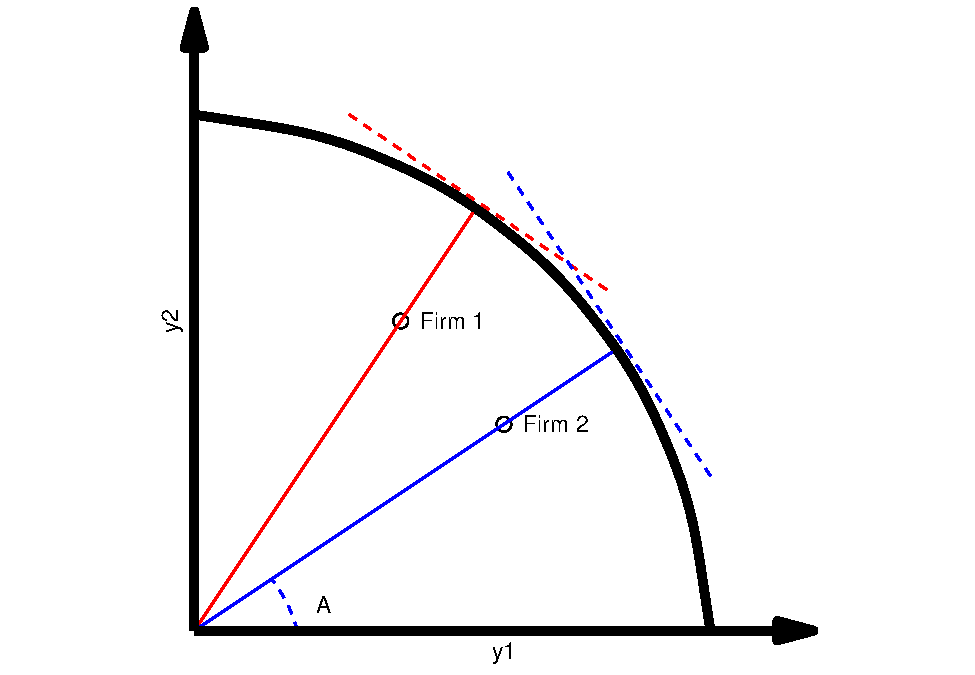
\includegraphics{EE_R-R_files/figure-pdf/fig-iso-1.pdf}

}

\caption{\label{fig-iso}Two output isoquant}

\end{figure}

\begin{footnotesize}

The figure represents a two output production model, where the black arc line is the best practice output frontier. Firm one and Firm two are operating below the frontier and are inefficient. These firms can improve their production efficiency (move towards the output frontier) by simultaneously producing more y2 and y1 for a given level of inputs (costs). Efficiency for each firm is the length of the dashed lines from the origin, the radial distance. The dashed tangents on the output frontier represent the shadow prices for the firms.

\end{footnotesize}

From figure Figure~\ref{fig-iso} , it is easy to see that the shadow
prices depend on both the curvature of the output isoquant and the
output mix, which the ratio y2/y1 can measure. Note that tan A = y2/y1,
where A is the angle indicated in figure Figure~\ref{fig-iso}. Note
further that the shadow prices depend on this angle (the polar
coordinates), **not** the distance to the frontier. Proportional scaling
of all outputs by some arbitrary constant along the dashed rays from the
origin does not affect the shadow prices.

What if we have empirically observed a change in the shadow prices (via
some regulatory or supervisory shock), and our objective is to test
whether this change is statistically significant? If the output isoquant
is held constant, the shadow prices can only change due to a change in
the output mix y2/y1. Therefore, we can test if there is a significant
change in the output mix. Note that the ratio y2/y1 is entirely
independent of the estimation of the frontier. Therefore, the test is
immune to possible serial correlation in the finite sample estimates of
the shadow prices. Some standard approaches to testing the significance
of the changes in the distribution of y2/y1 are reviewed in the next
section{[}\^{}15{]}

{[}\^{}15{]}: For completeness, it is worth noting that if the output
isoquant is linear (outputs are perfect substitutes in production), then
the shadow prices do not change even if the output mix changes. We could
test if the curvature of the output set is significant (i.e., if there
are significant economies of scope) by comparing the linear and convex
regression (see Meyer (2003) , for details), but this is not our primary
objective. Instead, we are interested in the effect of a change in the
regulatory and supervisory environment on shadow prices. This effect can
only occur through the change in the output mix.

Regulation can influence the output allocation, but not the economies of
scope or the shape of the production possibility set. Zhou, Zhou, and
Fan (2014) argues that a genuine objective of a production unit in the
presence of the introduction of a regulatory abatement target is to
reduce their undesirable output to the target level. If there is an
external abatement target, the producer primarily focuses on achieving
that target emissions level. After attaining this target, the economic
objective of the producer is to maximise the production of the desired
output to maximise profit. Thus, this external regulatory shock changes
the output allocation mix of desirable output to undesirable output but
not the shape of the production possibility set.

As a practical example, consider a regulatory shock that imposes a new
supervisory framework on a regulated system. In the efficiency
literature, regulatory externalities impose technological shifts to the
best-practice frontier technology (the solid line in figure
Figure~\ref{fig-iso}). If Hicks neutrality can be assumed, the effect on
the frontier is a parallel shift where the shape of the production
possibility set remains unchanged.

\hypertarget{references}{%
\section*{References}\label{references}}
\addcontentsline{toc}{section}{References}

\hypertarget{refs}{}
\begin{CSLReferences}{1}{0}
\leavevmode\vadjust pre{\hypertarget{ref-Anderson1952}{}}%
Anderson, T W, and D A Darling. 1952. {``Asymptotic Theory of Certain
{`Goodness of Fit'} Criteria Based on Stochastic Processes.''}
\emph{Ann. Math. Stat.} 23 (2): 193--212.

\leavevmode\vadjust pre{\hypertarget{ref-Anderson1954}{}}%
---------. 1954. {``A Test of Goodness of Fit.''} \emph{J. Am. Stat.
Assoc.} 49 (268): 765--69.

\leavevmode\vadjust pre{\hypertarget{ref-De_Angelis2019}{}}%
Angelis, Enrico Maria de, Marina Di Giacomo, and Davide Vannoni. 2019.
{``Climate Change and Economic Growth: The Role of Environmental Policy
Stringency.''} \emph{Sustain. Sci. Pract. Policy} 11 (8): 2273.

\leavevmode\vadjust pre{\hypertarget{ref-Bohringer2003}{}}%
Böhringer, Christoph, and Carsten Vogt. 2003. {``Economic and
Environmental Impacts of the Kyoto Protocol.''} \emph{Canadian Journal
of Economics/Revue Canadienne d'{é}conomique} 36 (2): 475--96.

\leavevmode\vadjust pre{\hypertarget{ref-Brechin2003}{}}%
Brechin, Steven R. 2003. {``Comparative Public Opinion and Knowledge on
Global Climatic Change and the Kyoto Protocol: The {US} Versus the
World?''} \emph{Int. J. Sociol. Soc. Policy} 23 (10): 106--34.

\leavevmode\vadjust pre{\hypertarget{ref-Brown1974}{}}%
Brown, Morton B, and Alan B Forsythe. 1974. {``Robust Tests for the
Equality of Variances.''} \emph{J. Am. Stat. Assoc.} 69 (346): 364--67.

\leavevmode\vadjust pre{\hypertarget{ref-Buonanno2003}{}}%
Buonanno, Paolo, Carlo Carraro, and Marzio Galeotti. 2003. {``Endogenous
Induced Technical Change and the Costs of Kyoto.''} \emph{Res. Energy
Econ.} 25 (1): 11--34.

\leavevmode\vadjust pre{\hypertarget{ref-Burniaux2000}{}}%
Burniaux, Jean-Marc. 2000. {``A Multi-Gas Assessment of the Kyoto
Protocol.''} \emph{OECD Economics Department Working Papers No. 270}.

\leavevmode\vadjust pre{\hypertarget{ref-Cifci2018}{}}%
Cifci, Eren, and Matthew E Oliver. 2018. {``Reassessing the Links
Between {GHG} Emissions, Economic Growth, and the {UNFCCC}: A
{Difference-in-Differences} Approach.''} \emph{Sustain. Sci. Pract.
Policy} 10 (2): 334.

\leavevmode\vadjust pre{\hypertarget{ref-Conover1999}{}}%
Conover, W J. 1999. \emph{Practical Nonparametric Statistics}. 3
edition. Wiley.

\leavevmode\vadjust pre{\hypertarget{ref-Dai.2020}{}}%
Dai, Sheng, Xun Zhou, and Timo Kuosmanen. 2020. {``{Forward-looking
assessment of the GHG abatement cost: Application to China}.''}
\emph{Energy Economics} 88: 104758.
\url{https://doi.org/10.1016/j.eneco.2020.104758}.

\leavevmode\vadjust pre{\hypertarget{ref-Fare2012}{}}%
Färe, Rolf, and Daniel Primont. 2012. \emph{{Multi-Output} Production
and Duality: Theory and Applications}. Springer Netherlands.

\leavevmode\vadjust pre{\hypertarget{ref-Fischer2006}{}}%
Fischer, Carolyn, and Richard D Morgenstern. 2006. {``Carbon Abatement
Costs: Why the Wide Range of Estimates?''} \emph{Energy J.} 27 (2):
73--86.

\leavevmode\vadjust pre{\hypertarget{ref-Gallagher2019}{}}%
Gallagher, Ronan, and Barry Quinn. 2019. {``Regulatory Own Goals: The
Unintended Consequences of Economic Regulation in Professional
Football.''} \emph{European Sport Management Quarterly}, April, 1--20.

\leavevmode\vadjust pre{\hypertarget{ref-Halkos2014}{}}%
Halkos, George E, and Nickolaos G Tzeremes. 2014. {``Measuring the
Effect of Kyoto Protocol Agreement on Countries' Environmental
Efficiency in {Co2} Emissions: An Application of Conditional Full
Frontiers.''} \emph{J Prod Anal} 41 (3): 367--82.

\leavevmode\vadjust pre{\hypertarget{ref-Hans-Jochen.2020}{}}%
Hans-Jochen, Luhmann, Sabine Balk, and Hans Dembowski. 2020. {``{Why
carbon emissions pricing and carbon shadow pricing both make sense}.''}
\emph{Development and Cooperation}.
\url{https://www.dandc.eu/en/article/why-carbon-emissions-pricing-and-carbon-shadow-pricing-both-make-sense/\#:/textbackslashtextasciitilde:text=Appropriate/\%20carbon/\%20prices/\&text=/\%E2/\%80/\%9CCarbon/\%20emissions/\%20pricing/\%E2/\%80/\%9D/\%20means/\%20that,not/\%20reflect/\%20those/\%20impacts/\%20yet.}

\leavevmode\vadjust pre{\hypertarget{ref-Hovi2012}{}}%
Hovi, Jon, Detlef F Sprinz, and Guri Bang. 2012. {``Why the United
States Did Not Become a Party to the Kyoto Protocol: German, Norwegian,
and {US} Perspectives.''} \emph{European Journal of International
Relations} 18 (1): 129--50.

\leavevmode\vadjust pre{\hypertarget{ref-Kumar.20207q}{}}%
Kumar, Surender, Shunsuke Managi, and Rakesh Kumar Jain. 2020. {``{CO2
mitigation policy for Indian thermal power sector: Potential gains from
emission trading}.''} \emph{Energy Economics} 86: 104653.
\url{https://doi.org/10.1016/j.eneco.2019.104653}.

\leavevmode\vadjust pre{\hypertarget{ref-Kuosmanen.2021}{}}%
Kuosmanen, Timo, and Xun Zhou. 2021a. {``{Shadow prices and marginal
abatement costs: Convex quantile regression approach}.''} \emph{European
Journal of Operational Research} 289 (2): 666--75.
\url{https://doi.org/10.1016/j.ejor.2020.07.036}.

\leavevmode\vadjust pre{\hypertarget{ref-Kousmanen.2021}{}}%
---------. 2021b. {``{Shadow prices and marginal abatement costs: Convex
quantile regression approach}.''} \emph{European Journal of Operational
Research} 289 (2): 666--75.
\url{https://doi.org/10.1016/j.ejor.2020.07.036}.

\leavevmode\vadjust pre{\hypertarget{ref-Kuosmanen.2020}{}}%
Kuosmanen, Timo, Xun Zhou, and Sheng Dai. 2020. {``{How much climate
policy has cost for OECD countries?}''} \emph{World Development} 125
(January): 104681. \url{https://doi.org/10.1016/j.worlddev.2019.104681}.

\leavevmode\vadjust pre{\hypertarget{ref-lee2014}{}}%
Lee, Sang-choon, Dong-hyun Oh, and Jeong-dong Lee. 2014. {``A New
Approach to Measuring Shadow Price: Reconciling Engineering and Economic
Perspectives.''} \emph{Energy Economics} 46: 66--77.
https://doi.org/\url{https://doi.org/10.1016/j.eneco.2014.07.019}.

\leavevmode\vadjust pre{\hypertarget{ref-Levene1961}{}}%
Levene, Howard. 1961. {``Robust Tests for Equality of Variances.''}
\emph{Contributions to Probability and Statistics. Essays in Honor of
Harold Hotelling}, 279--92.

\leavevmode\vadjust pre{\hypertarget{ref-Manne2004}{}}%
Manne, Alan, and Richard Richels. 2004. {``{US} Rejection of the Kyoto
Protocol: The Impact on Compliance Costs and {Co2} Emissions.''}
\emph{Energy Policy} 32 (4): 447--54.

\leavevmode\vadjust pre{\hypertarget{ref-McKibbin2004}{}}%
McKibbin, Warwick J, and Peter J Wilcoxen. 2004. {``Estimates of the
Costs of Kyoto: Marrakesh Versus the {McKibbin--Wilcoxen} Blueprint.''}
\emph{Energy Policy} 32 (4): 467--79.

\leavevmode\vadjust pre{\hypertarget{ref-Meyer2003}{}}%
Meyer, Mary C. 2003. {``A Test for Linear Versus Convex Regression
Function Using Shape‐restricted Regression.''} \emph{Biometrika} 90 (1):
223--32.

\leavevmode\vadjust pre{\hypertarget{ref-Nordhaus1999}{}}%
Nordhaus, William D, and Joseph G Boyer. 1999. {``Requiem for Kyoto: An
Economic Analysis of the Kyoto Protocol.''} \emph{Energy J.} 20:
93--130.

\leavevmode\vadjust pre{\hypertarget{ref-OBrien1981}{}}%
O'Brien, Ralph G. 1981. {``A Simple Test for Variance Effects in
Experimental Designs.''} \emph{Psychol. Bull.} 89 (3): 570--74.

\leavevmode\vadjust pre{\hypertarget{ref-Reilly1999}{}}%
Reilly, J, R Prinn, J Harnisch, J Fitzmaurice, H Jacoby, D Kicklighter,
J Melillo, P Stone, A Sokolov, and C Wang. 1999. {``Multi-Gas Assessment
of the Kyoto Protocol.''} \emph{Nature} 401 (6753): 549--55.

\leavevmode\vadjust pre{\hypertarget{ref-Rubin2015}{}}%
Rubin, Edward S, John E Davison, and Howard J Herzog. 2015. {``The Cost
of {Co2} Capture and Storage.''} \emph{Int. J. Greenhouse Gas Control}
40 (September): 378--400.

\leavevmode\vadjust pre{\hypertarget{ref-Stephens1986}{}}%
Stephens, Michael A. 1986. {``Tests Based on {EDF} Statistics.''} In
\emph{Goodness-of-Fit-Techniques}, 97--194. Routledge.

\leavevmode\vadjust pre{\hypertarget{ref-stiglitz2017report}{}}%
Stiglitz, Joseph E, Nicholas Stern, Maosheng Duan, Ottmar Edenhofer,
Gaël Giraud, Geoffrey M Heal, Emilio Lèbre La Rovere, et al. 2017.
{``Report of the High-Level Commission on Carbon Prices.''}

\leavevmode\vadjust pre{\hypertarget{ref-Tsionas.2022}{}}%
Tsionas, Mike G. 2022. {``{Convex Non-Parametric Least Squares, Causal
Structures and Productivity}.''} \emph{European Journal of Operational
Research}. \url{https://doi.org/10.1016/j.ejor.2022.02.020}.

\leavevmode\vadjust pre{\hypertarget{ref-Vale2016}{}}%
Vale, Petterson Molina. 2016. {``The Changing Climate of Climate Change
Economics.''} \emph{Ecol. Econ.} 121 (January): 12--19.

\leavevmode\vadjust pre{\hypertarget{ref-Viguier2003}{}}%
Viguier, Laurent L, Mustafa H Babiker, and John M Reilly. 2003. {``The
Costs of the Kyoto Protocol in the European Union.''} \emph{Energy
Policy} 31 (5): 459--81.

\leavevmode\vadjust pre{\hypertarget{ref-Welch1947}{}}%
Welch, B L. 1947. {``The Generalisation of Student's Problems When
Several Different Population Variances Are Involved.''}
\emph{Biometrika} 34 (1-2): 28--35.

\leavevmode\vadjust pre{\hypertarget{ref-Xian.2022}{}}%
Xian, Yujiao, Dan Yu, Ke Wang, Jian Yu, and Zhimin Huang. 2022.
{``{Capturing the least costly measure of CO2 emission abatement:
Evidence from the iron and steel industry in China}.''} \emph{Energy
Economics} 106: 105812.
\url{https://doi.org/10.1016/j.eneco.2022.105812}.

\leavevmode\vadjust pre{\hypertarget{ref-Zhang1998}{}}%
Zhang, Zhongxiang, and Henk Folmer. 1998. {``Economic Modelling
Approaches to Cost Estimates for the Control of Carbon Dioxide
Emissions.''} \emph{Energy Econ.} 20 (1): 101--20.

\leavevmode\vadjust pre{\hypertarget{ref-Zhou2014}{}}%
Zhou, P, X Zhou, and L W Fan. 2014. {``On Estimating Shadow Prices of
Undesirable Outputs with Efficiency Models: A Literature Review.''}
\emph{Appl. Energy} 130 (October): 799--806.

\end{CSLReferences}

\end{document}
